\chapter{Modelos DSGE}
%
%
\section{\citet{Neiss:2003}: The Real-Interest Rate gap as Inflation Indicator}
Este artigo examinou o que um modelo DSGE tem a dizer sobre o hiato da taxa de juros real como um indicador de inflação. Uma lacuna do conceito é que ele requer a construção de uma série de taxas reais naturais “não observáveis”. No entanto, o mesmo é verdade para o conceito de hiato do produto, e nossos resultados sugerem que a série do hiato do produto com frequência construída pode ser enganosa. Nessas circunstâncias, uma série de desvios da taxa de juros real é útil para avaliar a orientação da política monetária e a pressão inflacionária. Seus resultados sugerem que há benefícios em permitir movimentos da taxa natural ao modelar a inflação e basear a construção de séries de taxas naturais na teoria econômica. Os benefícios quantitativos podem ser modestos, entretanto, por causa do baixo grau de variação cíclica na taxa natural.

Este artigo desenvolve um modelo DSGE de preço fixo para examinar o comportamento da taxa de juros real natural e do gap da taxa de juros real. Todos os modelos DSGE fornecem implicitamente modelos do gap da taxa de juros real. Em modelos de preços flexíveis, o comportamento da diferença da taxa real é trivial - é zero a cada período porque a taxa de juros real é a taxa natural.

Incluímos a formação de capital e os choques de preferência, bem como outros elementos ausentes dos artigos acima, como a utilidade não separável no tempo. Também consideramos mais de uma especificação de definição de preço.

Os dois principais resultados deste artigo são que a taxa real natural não flutua muito ao longo do ciclo de negócios e, portanto, a taxa real é uma proxy razoável para a diferença da taxa de juros real; e que, em contraste, a variação do produto potencial é importante na frequência do ciclo de negócios. Esses resultados são consistentes com os pontos (i) e (ii) acima e têm implicações importantes para a modelagem da inflação e para as regras de política.

Sob preços flexíveis, as taxas de juros reais e naturais coincidem independentemente da regra de política monetária. Mas a política monetária tem efeitos reais quando os preços são rígidos, de modo que a especificação da regra de política terá implicações para a diferença da taxa de juros real. Examinamos as propriedades da diferença da taxa de juros real sob uma variedade de regras diferentes

Resposta da taxa natural de juros a choques de tecnologia e de preferência.
\begin{figure}[H]
\centering
%\includegraphics[scale=0.60]{Figura Neiss.jpg}
\includegraphics[scale=0.60]{Figuras/Figura Neiss.jpg}
%\caption {\tiny Taxa Natural de Juros}
\end{figure}

Tech shoch: No caso sem capital, um choque tecnológico aumenta a produção e o consumo hoje em mais do que em períodos futuros. A restrição de oferta agregada do período atual sobre a capacidade de consumo da família foi relaxada, e a restrição em períodos futuros foi relaxada por uma quantidade menor e decrescente. As famílias iriam gostar de suavizar seu consumo do produto mais alto (especialmente dada a formação de hábito em suas preferências) e tentam adiar muito de seu consumo mais alto. Mas, em equilíbrio, toda a produção deve ser consumida hoje. A taxa de juros real natural diminui para garantir que isso ocorra

Quando o capital pode variar, o investimento aumenta porque o choque tecnológico aumenta a lucratividade da produção. Isso tende a aumentar $r_t^{*}$. A pressão compensatória vem do desejo das famílias de economizar parte da renda extra e do desincentivo ao investimento rápido dos custos de ajuste. O efeito líquido é uma queda em $r_t^{*}$, embora menor do que no caso sem capital.

Preference shock: Ao contrário de um choque de política monetária, isso afeta os valores das variáveis reais sob a flexibilidade de preços. O choque aumenta a demanda de consumo. Com o capital totalmente flexível, apenas uma pequena mudança na taxa real é necessária para facilitar um declínio no investimento e abrir espaço para um consumo maior; portanto, a resposta limitada de $r_t^{*}$. Se não houver capital ou se as empresas enfrentarem grandes custos de ajuste, a taxa real deve aumentar mais para amortecer o aumento do consumo.

Agora nos voltamos para o caso do rigidez de preço e examinamos a resposta do gap da taxa de juros real. Resposta da taxa natural de juros a choques de tecnologia e de preferência.

\begin{figure}[H]
\centering
%\includegraphics[scale=0.60]{Figura Neiss2.jpg}
\includegraphics[scale=0.60]{Figuras/Figura Neiss2.jpg}
%\caption {\tiny Taxa Natural de Juros}
\end{figure}

O efeito de um choque tecnológico. O choque gera um aumento na diferença da taxa de juros real - um aperto de política eficaz - por dois motivos. Primeiro, a taxa natural cai e, portanto, para uma dada taxa de juros real, a política monetária é mais rígida. Em segundo lugar, a regra de política responde ao nível de produto e, portanto, um choque de produtividade induz um aumento na taxa de juros nominal e, portanto, real.

Um choque IS, entretanto, aumenta a taxa real e natural. Assim, em contraste com o caso do choque tecnológico, a resposta política - um aperto em resposta a um produto mais alto - tende a conter a abertura de um hiato da taxa real. No entanto, o aumento da taxa real é menor do que o aumento da taxa natural e, portanto, a orientação geral da política é mais frouxa.

Um aperto monetário afeta apenas a taxa de juros real. A diferença da taxa real, portanto, aumenta um por um com a taxa real. As respostas do produto e do hiato do produto são idênticas porque a política monetária não pode afetar o PIB potencial.

%
%
\section{\citet{Orphanides:2002}: Robust Monetary Policy Rules with Unknown Natural Rates }
Policymakers não conhecem os valores dessas taxas naturais em tempo real, isto é, quando tomam decisões políticas. De fato, mesmo em retrospectiva, há uma incerteza considerável em relação às taxas naturais de desemprego e juros, e ambiguidade sobre como melhor modelar e estimar as taxas naturais.

Esses problemas de mensuração parecem ser particularmente agudos na presença de mudanças estruturais quando as taxas naturais podem variar de maneira imprevisível, fazendo com que as estimativas das taxas naturais estejam sujeitas a um aumento da incerteza.

Empregamos um modelo trimestral foward-looking da economia norte-americana para examinar as propriedades de desempenho e robustez de regras de política de taxa de juros simples na presença de medidas precárias em tempo real das taxas naturais de juros e desemprego. Um aspecto fundamental de nossa investigação é o reconhecimento de que os formuladores de políticas podem estar incertos quanto aos verdadeiros processos geradores de dados que descrevem as taxas naturais de desemprego e juros e a extensão do problema de inconsistência que eles enfrentam. Como resultado, aplicações padrão de equivalência certeza baseadas no problema clássico de controle linear-quadrático-Gaussiano não se aplicam.

Nós achamos que os custos de subestimar a extensão da mensuração da taxa natural excedem significativamente os custos de superestimação. Adoção de regras de política otimizadas sob a falsa suposição de que as percepções errôneas em relação às taxas naturais provavelmente serão pequenas, o que é particularmente custoso em termos de estabilização da inflação e do desemprego.

Quando os formuladores de políticas não possuem uma estimativa precisa da magnitude das percepções errôneas em relação às taxas naturais, uma estratégia robusta é agir como se a incerteza que enfrentassem fosse maior do que suas estimativas básicas sugerem que pode ser. Mostramos que negligenciar essas considerações pode facilmente resultar em políticas com desempenhos de estabilização consideravelmente piores do que o previsto.

Nossos resultados apontam para uma estratégia simples e eficaz que é uma solução robusta para as dificuldades associadas às percepções errôneas da taxa natural. Isso é para adotar, como diretrizes para política monetária, regras de diferenças nas quais a taxa de juros nominal de curto prazo é aumentada ou diminuída de seu nível existente em resposta à inflação e mudanças na atividade econômica. Essas regras, que não requerem conhecimento das taxas naturais de juros e desemprego e, consequentemente, são imunes a percepções errôneas nesses conceitos, emergem como a solução para um exercício de controle robusto a partir de uma família mais ampla de especificações de regras de política.

Este artigo reexaminou criticamente a utilidade das taxas naturais de juros e desemprego no cenário da política monetária. Nossos resultados sugerem que subestimar a falta de confiabilidade das estimativas em tempo real das taxas naturais pode levar a políticas que são muito muito caras em termos do desempenho de estabilização da economia. De fato, nossas análises e conclusões são baseadas inteiramente em modelos em que os desvios das taxas naturais são os principais propulsores da inflação e do desemprego. Em vez disso, argumentamos que a incerteza sobre as taxas naturais em tempo real recomenda não depender excessivamente desses indicadores intrinsecamente ruidosos para decisões de política monetária.
%
%
\section{\citet{Edge:2008}: Natural rate measures in an estimated DSGE model of the U.S. economy  }
Estima um DSGE para economia dos EUA, utilizando de técnicas de econometria bayesiana. Eles usam seu modelo estimado para gerar e interpretar estimativas baseadas em modelo do produto potencial e a taxa natural de juros. Em modelos DSGE estimados como o nosso, os caminhos históricos para choques estruturais não observados são estimados além dos valores dos parâmetros. Consequentemente, podemos derivar estimativas históricas de variáveis de taxa natural, que, de maneira importante, têm interpretações estruturais muito claras.

Em sua discussão sobre nossas estimativas baseadas em modelo de produto potencial (e, portanto, o hiato do produto) e a taxa natural de juros, fornecemos vários exemplos de como nosso modelo pode auxiliar sua compreensão da macroeconomia dos EUA nos últimos 20 anos. Além disso, também consideramos como as estimativas do nosso modelo do hiato do produto e a taxa de juros natural diferem daquilo que consideramos como sabedoria convencional. Descobrimos que, embora a trajetória estimada do modelo da taxa natural de juros seja notavelmente mais volátil do que as estimativas derivadas (e nossa visão da sabedoria convencional), a trajetória estimada do modelo do hiato do produto compartilha algumas características importantes com outras produções mais tradicionais. estimativas baseadas em função.

A taxa natural de juros implícita em nosso modelo é muito volátil. Além de sua plausibilidade para os formuladores de políticas, pode haver mais questões relacionadas a flutuações na taxa de juros natural e seu papel no processo político em um modelo típico de DSGE como o nosso. Em particular, nosso modelo baseia-se na persistência de hábito para gerar respostas persistentes, em forma de hump-shaped, de variáveis-chave de gastos para os fundamentos. É bem sabido que essa especificação de preferências tem algumas implicações de preços de ativos intragáveis; Especificamente, esses modelos implicam substancial volatilidade na taxa de juros real livre de risco.
%
%
\section{\citet{Lopez-Salido:2009}: Money and the natural rate of interest: Structural estimates for the United States and the euro area }

Neste artigo, examinam o papel da moeda em uma estrutura geral que abrange três ambientes concorrentes: o modelo novo keynesiano  base com utilidade separável e demanda de moeda estática; utilidade inseparável entre o consumo e os saldos reais, juntamente com a formação de hábitos; e o modelo modificado para permitir custos de ajuste para manter os saldos reais. As duas últimas variantes implicam um caráter foward looking dos saldos monetários reais que transmite a moeda um papel importante como indicador de política monetária. o modelo padrão Novo Keynesian é um caso especial restritivo em que a moeda é menos informativo. Distinguimos entre esses cenários alternativos, realizando uma análise econométrica estrutural para os Estados Unidos e a área do euro. Nossas estimativas de probabilidade confirmaram o caráter foward looking da demanda por moeda. Uma das principais fontes desse comportamento voltado para o futuro é a existência de custos de ajuste de portfólio.

Ilustram como o valor da moeda aumenta em nos modelos estimados, em relação ao modelo base novo keynesiano, pela especificação da dinâmica da demanda por moeda para a qual encontramos suporte empírico. Nós nos concentramos nas ligações entre a moeda e a taxa natural e demonstramos que a moeda pode ter valor como um indicador de futuras variações na taxa natural, mesmo quando a dinâmica da inflação é vista através de uma estrutura neo-wickselliana do tipo defendido por Woodford (2003).

Neste artigo, distinguimos entre as visões alternativas do papel da moeda no mecanismo de transmissão, realizando uma análise econométrica estrutural das economias dos EUA e da área do euro. O modelo de equilíbrio geral estocástico dinâmico que estimado fornece cada variante de modelo  como um caso especial. Um resultado importante é que as estimativas de máxima verossimilhança confirmam o caráter prospectivo da demanda por moeda. Usando o modelo estimado, é capaz de demonstrar a capacidade aumentada da moeda para capturar o mecanismo de transmissão da política monetária quando a demanda por moeda tem um elemento prospectivo. Em particular, mostramos que o valor do dinheiro como proxy para as variações na taxa de juros natural e a diferença da taxa de juros real é aumentado.

A demanda por moeda é dada por:
$$\tilde{m}_t = \psi\tilde{m}_{t-1} + b_0 \tilde{y}_t + c_o \tilde{r}_t + \sum_{i=1}^{\infty} d_i E_t \tilde{rr^{*}}_t  \sum_{i=1}^{\infty} f_i E_t \{\tilde{rr}_{t+i} - \tilde{rr^{*}}_{t+i}  \} + \epsilon_t $$

Que toda a variação nos saldos reais não é decorrente de seus determinantes "convencionais" (ou seja, a renda real atual, a
taxa de juros de curto prazo atual, saldos defasados e o choque de demanda de moeda) está associado a movimentos nas defasagens de taxa de juros futura esperadas ou taxas de juros reais naturais esperadas. Notamos que a relação entre os saldos monetários reais e a taxa natural é bastante complexa, não apenas por causa da dinâmica envolvida, mas também porque a taxa natural entra com coeficientes negativos e positivos na expressão.

Essa perspectiva sobre a relação demanda por moeda destaca três vantagens da estimativa de nosso modelo estrutural por métodos de informação completa. Primeiro, as funções de demanda por moeda estimadas padrão negligenciam o comportamento prospectivo. O erro de especificação resultante ignora as informações sobre a taxa natural na demanda por moeda, em vez de atribuir a variação associada nos saldos reais a choques de demanda, ajustes defasados e respostas à renda corrente e à taxa de juros nominal. Nossa abordagem, ao contrário, isola o componente prospectivo da demanda por moeda e, portanto, oferece a perspectiva de uma estimativa consistente dos parâmetros de demanda monetária. Em segundo lugar, ao especificar explicitamente os processos de choque e o comportamento da política e, assim, o caminho implícito dos termos de expectativas que aparecem nas condições de otimalidade dos agentes, podemos extrair estimativas de taxa natural de outros determinantes inobserváveis da demanda de moeda. Terceiro, outras estimativas empíricas de séries de desvios de taxa natural e real utilizando métodos de sistemas, seja com modelos ad hoc (eg Laubach e Williams, 2003) ou modelos DSGE (eg Smets e Wouters, 2003), sacrificam informações sobre a taxa natural por não incluir saldos monetários reais no conjunto de variáveis modeladas. Nossas estimativas de sistemas, pelo contrário, incluem dinheiro na função de verossimilhança.

A taxa real de juros natural corresponde à taxa real de juros de curto prazo que prevaleceria quando a probabilidade Calvo se aproxima de 1,0, ou seja, quando todos os preços são flexíveis (e todas as empresas são foward looking). O processo de taxa natural será invariante à regra de política monetária, mas será uma função (possivelmente dinâmica) dos dois choques reais no modelo (IS (preferência) e choque tecnológico). Na aplicação aqui, a obtenção de uma série de taxa natural envolve a avaliação de nosso modelo com parâmetros que descrevem preferências e produção em seus valores estimados, resolvendo o modelo a preços flexíveis e obtendo uma representação ao estilo de Wold da taxa natural.

\section{\citet{Justiniano:2010}: Measuring the Equilibrium Real Interest Rate }

A taxa de juros real de equilíbrio é um conceito crucial na classe de modelos novo keynesianos. Essa taxa representa a taxa real de retorno necessária para manter a produção da economia igual à produção potencial, que, por sua vez, é o nível da produção consistente com preços e salários flexíveis e as constantes markup nos mercados de bens e de trabalho. Enquanto isso, a diferença entre a taxa de juros real ex ante - a taxa de juros nominal menos a inflação esperada - e a taxa de juros real de equilíbrio é definida como da taxa de juros real gap.

No modelo novo keynesiano, a diferença da taxa de juros real (RIR daqui em diante) é central para a determinação da taxa de juros e da inflação. Falando livremente, se essa lacuna do RIR for positiva, a produção diminuirá em relação ao potencial. Isso ocorre porque as pessoas estarão inclinadas a adiar as decisões de gastos hoje para aproveitar os maiores retornos da economia. Tudo o mais sendo igual, um hiato negativo do produto colocará pressões descendentes sobre os preços e os salários por causa da demanda agregada mais fraca. Por outro lado, um gap negativo do RIR estará tipicamente associado a um hiato positivo do produto, colocando em movimento as forças inflacionárias - uma demanda maior leva a preços mais altos.

O RIR de equilíbrio constitui uma referência natural para a condução da política monetária, e o gap do RIR pode ser visto como fornecendo alguma indicação da postura da política monetária. Embora o RIR de equilíbrio seja teoricamente atraente, seu uso na orientação de decisões de política monetária enfrenta pelo menos dois grandes obstáculos. Em primeiro lugar, o RIR de equilíbrio não é diretamente observável nos dados, limitando sua utilidade como um meta para a política monetária na prática. O RIR de equilíbrio flutua ao longo do tempo em resposta a uma variedade de choques nas preferências e na tecnologia que perturbam a economia.

Segundo, definir taxas de juros nominais para rastrear o RIR de equilíbrio pode não ser viável às vezes devido à existência do zero bound; isto é, as taxas de juros nominais não podem ser definidas abaixo de zero. De fato, o RIR de equilíbrio pode cair o suficiente para induzir um gap positivo no RIR, mesmo com a taxa de juros nominal em zero. A produção cairia abaixo do potencial, gerando deflação. Desta forma, a diferença nos ajuda a medir a restrição imposta pelo zero ligado à política monetária. Com taxas de juros nominais de curto prazo agora em níveis historicamente baixos nos Estados Unidos e em vários outros países industrializados, esse cenário está recebendo muita atenção tanto da comunidade acadêmica quanto dos formuladores de políticas.

Dada a importância que o RIR de equilíbrio desempenha para o desenho da política monetária em modelos macroeconômicos modernos, nosso objetivo neste artigo é fornecer uma estimativa dessa variável não observável. Fazemos isso inferindo-o de um novo modelo keynesiano empírico adaptado aos dados trimestrais dos EUA. 

Especificamente, nossa análise realiza três objetivos. Primeiro, descrevemos a evolução histórica do RIR de equilíbrio. Descobrimos que essa taxa foi negativa às vezes, particularmente no final da década de 1970 e, o mais interessante, durante a última recessão.

Além disso, estimamos o gap de curto prazo do RIR como a diferença entre o RIR ex ante atual (em oposição ao futuro) e o RIR de equilíbrio. Isso fornece algumas indicações sobre a postura da política monetária. Em consonância com a visão anedótica, a estimativa do gap do RIR de curto prazo sugere que a política foi frouxa durante a maior parte da década de 1970. Em contraste, a política parece ter sido apertada no final da nossa amostra. No entanto, isso reflete principalmente o problema do zero bound - incapacidade dos formuladores de políticas de reduzir as taxas de juros nominais de curto prazo abaixo de zero - e fornece uma justificativa para as medidas não convencionais adotadas pelo Federal Reserve durante a recessão mais recente, como compras diretas de de curto prazo e criação de instalações e programas especiais

Por fim, comparamos a evolução o gap de curto prazo e de curto prazo dos RIRs, onde a última é definida como a soma dos gaps de curto prazo atuais e futuras de RIR ou, alternativamente, a diferença entre os RIR ex-ante de longo prazo e o RIR de longo prazo de equilíbrio. As taxas de longo prazo refletem a trajetória das taxas de curto prazo atuais e futuras esperadas. Portanto, os gaps de longo prazo resumem as expectativas privadas sobre os resultados macroeconômicos futuros e a política monetária, fornecendo uma medida mais voltada para o futuro da orientação da política. Por exemplo, de acordo com esta medida, a política não foi frouxa no período de 2002-2006, que precedeu a recente desaceleração econômica. Essa caracterização da postura da política contrasta com o que é sugerido pelo gap de curto prazo do RIR.

Neste artigo, estudamos a evolução dos desvios RIR e RIR de equilíbrio, usando tanto um novo modelo keynesiano prototípico quanto um modelo de escala maior. Nossas estimativas apontam para um grau substancial de variação no tempo no RIR de equilíbrio. Além disso, descobrimos que essa taxa às vezes se tornou negativa no período pós-guerra. Em particular, nossa análise sugere que o RIR de equilíbrio caiu acentuadamente abaixo de zero no final de 2008.

Concluímos observando que os modelos que usamos aqui, mesmo os de maior escala, são até certo ponto muito estilizados e apresentam algumas deficiências. Uma dessas deficiências é a ausência de uma estrutura teórica explícita do setor financeiro e das fricções financeiras.

Equações:
\begin{equation*} E_{t} \sum_{s=0}^{\infty} \beta^{s} b_{t+s}\left[\log C_{t+s}-\varphi \frac{L_{n+s}(j)^{1+v}}{1+v}\right]\end{equation*}


sujeito a: 
\begin{equation*}P, C_{t}+T_{t}+B_{t} \leq R_{t-1} B_{t-1}+Q_{t+1}(j)+\prod_{t}+W_{t}(j) L,(j)\end{equation*}


Rigidez de salário:
\begin{equation*}E_{t} \sum_{s=0}^{\infty} \xi_{w}^{s} \beta^{s} b_{t+s}\left\{-\varphi \frac{L_{t+t}(j)^{1+v}}{1+v}\right\}\end{equation*}

Labor input é homogeneo:
$L_{t}=\left[\int_{0}^{1} L_{t}(j)^{\frac{1}{1+\Lambda_{w} t} t} d j\right]^{1+\Lambda_{w, t}}$

Problema de maximizaçao e de lucro 0: 
$L_{t}(j)=\left(\frac{W_{t}(j)}{W_{t}}\right)^{-\frac{1+\Lambda_{w, t}}{\Lambda_{w, t}}} L_{t}$

Produtores de bens intermediários:
$Y_t(i) = A_tL_t(i)^{\alpha}$

Rigidez a la Calvo: $$
E_{t} \sum_{s=0}^{\infty} \xi_{p}^{s} \beta^{s} \Lambda_{t+s}\left\{\left[\tilde{P}_{t}(i) \pi^{s}\right] Y_{t+s}(i)-W_{t+s} L_{t+s}(i)\right\}
$$

Perfectly competitive firms produce the final good
$Y_{t}$ by bundling all intermediate goods according to
$$
Y_{t}=\left[\int_{0}^{1} Y_{t}(i)^{\frac{1}{1+\lambda_{p} t} d i}\right]^{1+\Lambda_{p} t}
$$
Profit maximization and zero profit condition for the final goods producers imply the following demand function for the intermediate good $i$
$$
Y_{t}(i)=\left(\frac{P_{t}(i)}{P_{t}}\right)^{-\frac{1+\Lambda_{p, t}}{\Lambda_{p, t}}} Y_{t}
$$

Regra de Política Monetária:
\begin{equation}\frac{R_{t}}{R}=\left(\frac{R_{t-1}}{R}\right)^{\rho_{x}}\left[\left.\left(\frac{\left(\begin{array}{l}
3 \\
\prod_{s=0} \pi_{t-s}
\end{array}\right)^{1 / 4}}{\pi_{t}^{*}}\right)^{\phi_{\tau}}\left(\frac{\left(Y_{t} / Y_{t-4}\right)^{1 / 4}}{e^{\gamma}}\right)^{\phi_{y}}\right|^{1-p_{R}} e^{\varepsilon_{R_{R}}}\right.\end{equation}
%
%
\section{\citet{Bjornland:2011}: Estimating the natural rates in a simple New Keynesian framework  }

O objetivo principal deste artigo é apresentar um arcabouço simples para derivar as taxas naturais dentro de um cenário de modelo novo keynesiano. O modelo é pequeno, mas incorpora os principais ingredientes da estrutura novo keynesiana, tornando-se um instrumento útil para analisar como as mudanças nas taxas naturais afetam a economia e a política monetária. Apesar da natureza simples do modelo, derivamos estimativas plausíveis de variação de tempo das taxas naturais e as taxas de juros e hiatos do produto correspondentes usando estimativas bayesianas e técnicas de filtro de Kalman nos dados dos EUA.

Este artigo fornece estimativas da taxa de juros real natural, do hiato do produto e da meta implícita de inflação para a economia dos EUA. A meta de inflação desde 1994 tem sido notavelmente estável em torno de 2$\%$. A taxa de juros real natural, no entanto, tem variado muito.

Ao estimar a curva híbrida New Keynesian Phillips com uma estimativa consistente do modelo do hiato do produto, descobrimos que a estrutura da curva é muito semelhante àquela encontrada pela estimativa da curva de Phillips com a participação do trabalho na renda. Nossos resultados são, portanto, uma contribuição para o debate sobre se é o hiato do produto ou a participação do trabalho na renda, que fornece a melhor representação para o processo de inflação.

Nossa abordagem é, no entanto, uma reserva em relação a uma abordagem DSGE completa, na medida em que não impomos restrições tecnológicas nem modelamos o mercado para fatores de produção. O lado da oferta da economia é governado por processos exógenos. Outra faceta da contribuição deste artigo é a concessão da possibilidade de uma meta de inflação variável no tempo. Uma terceira novidade da nossa abordagem é que ela não exige detrending os dados antes da análise (usando, por exemplo, o filtro HP) ou torna o produto estacionário deflacionando por uma variável de tendência.

O que o modelo deles tem de diferente do Gali (2015).

Consumidor: Hábito externo, com persistência de segunda ordem $H_t = C_{t-1}^{\gamma_1}C_{t-2}^{\gamma_2}$. Isso gera a seguinte IS Curve: $\Delta y_t = \dfrac{\sigma}{\gamma_1(\sigma -1 )}E_t \Delta y_{t+1} - \dfrac{\gamma_2}{\gamma_1}\Delta y_{t-1} - \dfrac{1}{\gamma_1 (\sigma -1)}(i_t - E_t \pi_{t+1} - \rho) + \dfrac{1}{\gamma_1}(\upsilon_t - E_t \upsilon_{t+1}) $. O choque de preferência no consumo: $\upsilon_t = \rho_{\upsilon}\upsilon_{t-1} + \epsilon_t^{\upsilon} $. \\

Oferta Agregada. Curva de Phillips híbrida, que incorpora foward-looking e backward-looking $\pi_t = \mu E_t \pi_{t+1} + (1 - \mu) \sum_{j=1}^{4} \alpha_j \pi_{t-j} + \kappa x_t + \epsilon_t^{\pi} $.Hiato do produto $x_t = y_t - y_t^{n}$. A taxa natural do produto é dado por um processo exógeno: $\Delta y_t^{n} = \upsilon + \omega_t $. Aqui $\omega_t$ é o choque na taxa de crescimento (choque na taxa natural) $\omega_t = \phi \omega_{t-1} + \varrho_t $. O hiato do produto segue o seguinte processo $x_t = x_{t-1} + \Delta y_t - \Delta y_t^{n} $.\\

Política Monetária. Regra de Taylor $i_t = \psi i_{t-1} + (1 - \psi)(i_t^{n} + \theta_{\pi}(\bar{\pi}_t - \pi_t^{T}) + \theta_x x_t ) + \epsilon_t^{i} $, $i_t^{n}$ é a taxa natural nominal de juros, $\bar{\pi}_t = \dfrac{1}{4} \sum_{j=0}^{3} \pi_{t-j}$, a meta de inflação varia ao longo do tempo $\pi_t^{T} = (1 - \rho_{\pi}) \pi^{*} + \rho_{\pi}\pi_{t-1}^{T} + \xi_t$ e $\xi_t $ é um AR(1) choque na meta de inflação $\xi_t = \rho_{\xi}\xi_{t-1} + \epsilon_t^{\xi}$.\\

A taxa natural de juros. Pode ser obtida a partir da IS Curve $\Delta y_t^{n} = \dfrac{\sigma}{\gamma_1(\sigma -1 )}E_t \Delta y_{t+1}^{n} - \dfrac{\gamma_2}{\gamma_1}\Delta y_{t-1}^{n} - \dfrac{1}{\gamma_1 (\sigma -1)}(i_t^{n} - E_t \pi_{t+1} - \rho) + \dfrac{1}{\gamma_1}(\upsilon_t - E_t \upsilon_{t+1}) $. Isolando a taxa natural de juros $i_t^{n} = \delta + E_t \pi_{t+1} + \sigma \Delta E_t y_{t+1}^{n} - \gamma_1 (\sigma -1) \Delta y_t^{n} - \gamma_2(\sigma -1) \Delta y_{t-1}^{n} + (\sigma -1)(\upsilon_t - E_t \upsilon_{t+1}) $. A taxa de juros real natural $ r_t^{n} = i_t^{n} - E_t \pi_{t+1}$. O hiato do produto pode ser obtido subtraindo a IS Curve da IS Curve do produto natural $ x_t = \dfrac{\sigma}{A}E_t x_{t+1} + \dfrac{(\gamma_1 - \gamma_2)(\sigma -1 )}{A}x_{t-1} + \dfrac{\gamma_2(\sigma -1)}{A}x_{t-2} - \dfrac{1}{A}(i_t - i_t^{n}) $.
%
%
\section{\citet{Melosi:2015}: The Natural Rate of Interest and Its Usefulness for Monetary Policy }

Interessante desse artigo é eles explicando o que é NRI em um modelo DSGE. Eles usam como modelo base, o livro do Gali. Em resumo, da IS Curve temos: $y_y = E_t y_{t+1} - s(i_t - E_t \pi_{t+1} - \rho_t ) - 0,5 s^{-1}\text{var}_t[y_{t+1}] $. A taxa natural de juros deve satisfazer $E_t[\Delta y_{t+1}^{n}] = s(r_t^{n} - \rho_t) + 0,5s^{-1}\text{var}_t[y_{t+1}] $. Resolvendo algebricamente $r_t^{n} = \rho_t + s^{-1}E_t[\Delta y_{t+1}^{n}] - 0,5s^{-2}\text{var}_t[y_{t+1}]$. Definição de produto natural $y_t^{n} = \psi_{ya}^{n}a_t + \vartheta_y^{n} $. Portanto a definição de taxa natural de juros: $r_t^{n} = \rho_t + s^{-1}\psi_{ya}^{n} E_t[\Delta a_{t+1}] - 0,5s^{-2}(\psi_{ya}^{n})^{2}\text{var}_t[a_{t+1}]$. O hiato do produto é $\tilde{y}_t = y_t - y_t^{n} $. Com isso, podemos chegar em $\tilde{y}_t = -s \sum_{k=0}^{\infty} E_t(r_{t+k} - r_{t+k}^{n}) $. A última expressão torna evidente que o hiato do produto é a soma de todos os hiatos da taxa de juros reais futuros, definidos como os desvios da taxa real ex ante, $i_t - E_t(\pi_{t+1})$ da taxa natural, $r_{t}^{n} $.

O que afeta a taxa natural de juros:
\begin{itemize}
    \item A taxa natural de juros é crescente na taxa de preferência, $\rho_t$ e a expectativa de crescimento da taxa de tecnologia $E_t[\Delta a_{t+1}] $ e decrescente na variância condicional da tecnologia futura $\text{var}_t[a_{t+1}] $.
    \item Uma trajetória da taxa de juro em que a taxa real real é sempre igual à taxa natural atinge tanto um hiato do produto de zero (no sentido em que o produto é igual ao natural, isto é, nível de equilíbrio de preço flexível) como a inflação igual a zero.
\end{itemize}

Eles baseiam-se no conhecido framework de Smets e Wouters (2007), que se mostrou adequado aos dados. Um modelo DSGE razoavelmente rico indica que, desde 1990, a taxa de juros real natural, definida como a taxa real de uma economia eficiente, sem rigidez nominal nem distorções de cost-push, tem sido bastante variável e altamente pró-cíclica. Eles descobrem que a taxa natural poderia ser uma estatística sumária útil para o FED, na medida em que a política projetada para rastreá-la estabilizaria significativamente o produto e falhas ineficientes, ao mesmo tempo em que diminuiria a variabilidade da inflação de preços e salários. No entanto, o limite inferior zero da taxa de juros e a dificuldade de calcular a taxa natural em tempo real impõem desafios não triviais à adoção da taxa de juros natural como meta implementável da política monetária.

Ao contrário do modelo canônico na primeira parte do artigo, uma economia mais rica, que está sujeita a choques de oferta ineficientes (por exemplo, choques de markup ou outros choques cost-push), não parece ter uma definição única e inequívoca do taxa de juros (ou produto). Pode-se definir a taxa natural como a taxa que prevaleceria se os salários e os preços fossem perfeitamente flexíveis. No entanto, se choques cost-push - também conhecidos como choques de markup - criam ineficiências, o equilíbrio de salários e preços flexíveis associados não seria "relevante para o bem-estar". Assim, em nosso modelo empírico, escolhemos definir a taxa de juros real e o nível de produto reais, como aqueles que teriam prevalecido em uma economia sem rigidez nominal nem choques nas margens de preço e de salário.

Estimativas da taxa natural (trimestralmente), que segue uma padrão altamente procíclico caracterizado por variações bastante pronunciadas. Talvez surpreendentemente, não observamos uma queda substancialmente maior durante a Grande Recessão do que nas duas desacelerações anteriores. No entanto, em contraste com recessões anteriores, manteve-se persistentemente negativo desde 2008. Este último achado é explicado principalmente pelo choque de risco negativo altamente persistente que, de acordo com o nosso modelo, desencadeou a Grande Recessão e é responsável pela lenta recuperação.
%
%
\section{\citet{Canzoneri:2015}: Monetary Policy and the Natural Rate of Interest}

Neste artigo, mostramos que o rastreamento da taxa natural também é importante para o bem-estar do household. Além disso, mostramos que é mais importante em um ambiente em que as taxas de juros tomam grandes e persistentes oscilações em torno de seus valores de equilíbrio de longo prazo, e é difícil para as regras de política monetária padrão fazer com que a taxa de juros alcance sua taxa natural. Usamos dois modelos para ilustrar esse fato: em um - que chamamos de Modelo Padrão (Novo Keynesiano) - as oscilações na taxa natural são substanciais, mas são de curta duração. No outro modelo - que chamamos de Modelo de Liquid Bonds - as oscilações podem ser maiores e muito mais persistentes. A razão é que os títulos do governo fornecem liquidez nesse modelo. Assim, um aumento no gasto público que é (inicialmente) financiado pela dívida proporcionará liquidez adicional neste modelo, gerando movimentos prolongados na demanda do consumidor e taxas de juros de equilíbrio. Mostraremos que o rastreamento da taxa natural é muito mais importante para o bem-estar do household no Modelo de Liquid Bonds. Em qualquer um dos modelos, os desvios da taxa de juros da taxa natural dependerão da política monetária vigente. Consideram 4 regras de Taylor:

\begin{align}
    \textsf{Regra 1 (regra básica de Taylor): }  i_t = \bar{i} + 1,5(\pi_t - \bar{\pi})  \\
    \textsf{Regra 2 (regra suavizada de Taylor): } i_t = 0,8i_{t-1} + 0,2[\bar{i} + 1,5(\pi_t - \bar{\pi}) ] \\
    \textsf{Regra 3 (regra primeira diferença): } i_t = i_{t-1} + 1,5(\pi_t - \bar{\pi}) \\
    \textsf{Regra 4 (regra da taxa natural): } i_t = [r_r^{n} + E_t(\pi_{t+1})] + 1,5(\pi_t - \bar{\pi}) 
\end{align}

A regra 4 é uma variante da regra de taxa natural discutida acima e funciona muito bem em ambos os nossos modelos. No entanto, a regra 4 pressupõe que a taxa natural é conhecida em todos os períodos. Como a taxa natural não é observada na prática, vemos a Regra 4 como a referência pela qual mais regras operacionais devem ser julgadas.

As regras 1 e 2 são regras convencionais de Taylor que foram estudadas extensivamente na literatura. Acredita-se que estejam operacionais, uma vez que apenas assumem que o valor de equilíbrio de longo prazo da taxa natural é conhecido. Essas regras demonstraram fornecer uma boa descrição empírica das políticas monetárias usadas por muitos bancos centrais e são frequentemente usadas em exercícios de avaliação de políticas. A Regra 3 não se enquadra na classe das regras convencionais de Taylor, e não temos conhecimento de qualquer literatura empírica, ou declaração do banco central, sugerindo que ela tenha sido seguida na prática. No entanto, essa primeira regra de diferença seria claramente implementável; na verdade, nem sequer exige o valor de equilíbrio de longo prazo da taxa natural.

No Modelo Padrão, a diferença na utilidade do household entre a Regra 1 e a Regra 4 vale 0,25$\%$ do consumo de estado estacionário a cada período, o que é um número substancial na literatura novo keynesiana. Em nossa calibração de referência do Modelo de Liquid Bonds, a diferença aumenta para 0,5$\%$ do consumo a cada período. Dinheiro e títulos são complementos na calibração de benchmark; tomamos nosso valor pela elasticidade de substituição entre dinheiro e títulos de uma estimativa de uma das equações do modelo. No entanto, nossas estimativas não são muito precisas e mostramos que, se em vez disso dinheiro e títulos fossem substitutos, então a diferença de utilidade entre a Regra 1 e a Regra 4 poderia estar mais próxima do que encontramos no Modelo Padrão. Finalmente, mostramos que a Regra 3 faz o melhor trabalho de rastrear a taxa natural após os quatro ou cinco trimestres iniciais, e ela executa quase tão bem quanto a Regra 4 em termos de utilidade doméstica. Achamos que a razão para isso é que, estando livre de um termo fixo de interceptação, a taxa de juros é livre para se mover amplamente ao longo do tempo.

Antes de proceder à análise, devemos abordar uma questão que está no centro do nosso trabalho: os títulos realmente têm valor de liquidez? A premissa básica não deve ser controversa. Os Treasuries dos EUA facilitam as transações de várias maneiras: servem como garantia em muitos mercados financeiros, os bancos os detêm para administrar a liquidez de seus portfólios e os indivíduos os mantêm em contas do mercado financeiro que oferecem serviços de verificação.

Há uma lição oportuna a ser aprendida em nossa análise. Até o momento, muitos países da OCDE estão empreendendo, ou contemplando, grandes cortes nos gastos do governo para estabilizar suas dívidas soberanas. Se os títulos fornecem serviços de liquidez, nossos resultados sugerem que a taxa de juros natural estará em movimento e difícil de acompanhar. A primeira regra de diferença parece ser feita apenas para esta situação.
%
%
\section{\citet{Curdia:2015}: Has U.S. monetary policy tracked the efficient interest rate? }

Este artigo propõe uma caracterização alternativa dos fatores que influenciam a evolução da FFR. Sua principal conclusão é que as regras de política em que a taxa de juros é definida para acompanhar uma medida da taxa real eficiente - a taxa de juros real que prevaleceria se a economia fosse perfeitamente competitiva - ajustam os dados melhor do que as regras nas quais o hiato do produto é a medida primária da atividade econômica real. Referimo-nos ao primeiro como regras W, de Wicksell (1898), que, notoriamente, definiu o problema da política monetária como uma tentativa de rastrear uma taxa de juros “neutra”, determinada apenas por fatores reais.

Avaliar até que ponto este tipo de raciocínio teve um impacto mensurável na evolução observada das taxas de política nos EUA requer um modelo estrutural, uma vez que a taxa real de equilíbrio é um objeto contrafactual. Calculamos esse contrafactual em duas variantes do modelo DSGE New Keynesian padrão com concorrência monopolística e preços rígidos, estimados em dados da Taxa de Fundos Federais (FFR), inflação e crescimento do PIB, como na literatura empírica sobre regras de Taylor. Dentro desse quadro, definimos o potencial de produção como o nível eficiente de produção agregada $y_t^{e}$, por exemplo, para que a taxa real de equilíbrio que “manteria a economia em seu potencial de produção” é a taxa eficiente de retorno $r_t^{e}$. Essa taxa de juros é eficiente porque é a que prevaleceria se os mercados fossem perfeitamente competitivos, em vez de distorcidos pelo poder de monopólio e pela dispersão de preços.

Além de apontar as regras W como uma ferramenta promissora para descrever a definição de taxas de juros na prática, nossos resultados também sugerem que esse componente, muitas vezes negligenciado, dos modelos estruturais pode ter um impacto significativo em sua adequação. A diferença nas probabilidades marginais entre as melhores e piores regras de ajuste consideradas neste estudo pode chegar a 50 log-points. Como referência, essas diferenças no ajuste são de uma ordem de magnitude similar àquelas entre modelos estruturais estimados com ou sem volatilidade estocástica. Esta evidência, portanto, ressalta a importância para os pesquisadores do DSGE de prestar muita atenção à especificação da política monetária.

Este artigo propõe uma visão alternativa dos fatores reais que impulsionam as decisões da taxa de juros. Regras nas quais o instrumento de política rastreia a taxa de juros eficiente como a medida principal dos desenvolvimentos econômicos reais se encaixam melhor nos dados do que as especificações equivalentes que respondem ao hiato do produto. Referimo-nos a essa classe de regras como regras W, de Wicksell (1898), cuja taxa de juros neutra é precursora da taxa eficiente de retorno aqui considerada.

Como essa taxa eficiente é um objeto contrafatual - a taxa de retorno que prevaleceria sob competição perfeita -, sua medição requer um modelo estrutural. Portanto, conduzimos nossa investigação empírica dentro de uma estrutura DSGE New Keynesian, usando métodos Bayesianos para estimar seus parâmetros e comparar o ajuste de muitas especificações alternativas. Em todas essas especificações, que diferem para os detalhes da regra de política, bem como para as suposições sobre o comportamento do setor privado, as regras W provaram-se consistentemente superiores às regras de Taylor equivalentes.

Apesar de sua robustez, este resultado está sujeito a duas ressalvas. Em primeiro lugar, a especificação do modelo é importante, pois nosso critério de ajuste depende da interação da regra de política com o restante do modelo. Mais trabalho entre diferentes modelos seria, portanto, desejável, embora já abordemos essa questão ilustrando a robustez dos resultados em duas especificações DSGE populares. Em segundo lugar, a comparação de modelos através de densidades de dados marginais e os fatores de Bayes aplicados aos modelos DSGE está sujeita a algumas armadilhas, destacadas, por exemplo, por Del Negro e Schorfheide (2011). No entanto, as grandes melhorias no ajuste descoberto ao passar das regras W para T sugerem que a especificação da função de reação a políticas faz uma diferença significativa.

IS Curve:
\begin{equation}
    \tilde{x}_t = E_t(\tilde{x}_{t+1}) - \varphi_{\gamma}^{-1}(i_t - E_t(\pi_{t+1}) - r_t^{e} )
\end{equation}

o nível de atividade corrente é $\tilde{x}_t \equiv (x_t^{e} - \eta_{\gamma}x_{t-1}^{e} ) - \beta \eta_{\gamma} E_t(x_{t+1}^{e} - \eta_{\gamma} x_t^{e} ) $ depende da expectativa futura da atividade real e do gap entre a taxa real ex-ante e seu nível eficiente, $x_t^{e} \equiv y_t - y_t^{e} $ é o hiato do produto.

NKPC:
\begin{equation}
    \tilde{\pi}_t = \xi(\omega x_t^{e} + \varphi_{\gamma}\tilde{x}_t ) + \beta E_t \tilde{\pi}_{t+1} + \upsilon_t
\end{equation}

a medida de inflação corrente: $\tilde{\pi}_t = \pi_t - \varsigma \pi_{t-1} $.

No entanto, fornece uma descrição razoável dos dados sobre o PIB, a inflação e a taxa de juros - as séries que são normalmente consideradas na estimativa das regras de taxa de juros. Outra vantagem de trabalhar com uma especificação de linha de base simplificada é que ela permitiu explorar a robustez das principais descobertas do documento em um grande número de regras de taxa de juros, sem ter que se preocupar com restrições computacionais.

O produto eficiente, indicado por $y_{t}^{e}$, e a taxa de juros real eficiente, indicada por $r_{t}^{e}$, são construções centrais em nossa análise. Eles representam os níveis de produção e da taxa de juros real que seriam observados em uma economia contrafactual na qual (i) os preços são - e sempre foram - flexíveis e (ii) as marcações desejadas são zero. Em nossa estrutura, essas premissas resultam em uma economia perfeitamente competitiva, o que proporcionaria uma alocação eficiente.

Produto eficiente evolui de acordo com:
$\omega y_{t}^{e}+\varphi_{\gamma}\left(y_{t}^{e}-\eta_{\gamma} y_{t-1}^{e}\right)-\beta \varphi_{\gamma} \eta_{\gamma}\left(E_{t} y_{t+1}^{e}-\eta_{\gamma} y_{t}^{e}\right)=\varphi_{\gamma} \eta_{\gamma}\left(\beta E_{t} \gamma_{t+1}-\gamma_{t}\right)+\frac{\beta \eta_y}{1-\beta \eta_{\gamma}} E_{t} \delta_{t+1}$

The intertemporal Euler equation implies
$r_{t}^{e}=E_{t} \gamma_{t+1}+E_{t} \delta_{t+1}-\omega E_{t} \Delta y_{t+1}^{e}$

Observamos que a taxa real eficiente depende positivamente dos componentes previsíveis do crescimento da produtividade $\gamma_{t+1}$ e do choque de preferência do próximo período $\delta_{t+1}$, e negativamente daqueles da taxa de crescimento da produção eficiente, $\y_{t+1}^{e}$. Intuitivamente, um aumento no desejo das famílias de consumir precocemente, capturado por um aumento persistente de $\delta_{t}$, pressiona a taxa real eficiente, de modo a dissuadir os consumidores de agir de acordo com seu desejo de antecipar o consumo. Da mesma forma, o maior crescimento esperado da produtividade requer perfis de consumo mais acentuados e, portanto, uma taxa real mais alta. Finalmente, o último termo capta o efeito negativo sobre a taxa de juros de uma taxa de crescimento esperada mais alta da utilidade marginal, que no equilíbrio eficiente está conectada à taxa de crescimento de horas e, portanto, da produção.

Regras de Política Monetária.

Regra W
\begin{equation}
    i_t = \rho i_{t-1} + (1 - \rho)(r_t^{e} + \phi_{\pi} \pi) + \epsilon_t^{i}
\end{equation}

Regra T
\begin{equation}
    i_t = \rho i_{t-1} + (1 - \rho)(\phi_{\pi} \pi + \phi_x x_t^{e}) + \epsilon_t^{i}
\end{equation}
%
%
\section{\citet{Del-Negro:2015}: Inflation in the Great Recession and New Keynesian Models}

Neste artigo, usamos um modelo DSGE padrão, que estava disponível antes da recente crise e que é estimado com dados até 2008, para explicar o comportamento do crescimento do produto, inflação e custos marginais desde a crise. O modelo utilizado é o modelo de Smets e Wouters (2007), baseado em Christiano, Eichenbaum e Evans (2005), estendido para incluir fricções financeiros como em Bernanke, Gertler e Gilchrist (1999), Christiano, Motto e Rostagno (2003), e Christiano, Motto e Rostagno (2014).

Mostramos que, assim que o estresse financeiro salta no outono de 2008, o modelo prevê com sucesso uma forte contração na atividade econômica, juntamente com um declínio relativamente modesto e prolongado da inflação. As mudanças de preço são projetadas para permanecer na vizinhança de 1$\%$. Esse resultado contrasta com a afirmação de Hall (2011), Ball e Mazumder (2011), e outros de que os modelos neo-keynesianos estão fadados a não captar os amplos contornos da Grande Recessão e a quase estabilidade da inflação.

Segundo o NKPC, a inflação é determinada pela soma descontada dos custos marginais esperados no futuro (inflação fundamental). A chave para entender nosso resultado é que a inflação é mais dependente dos custos marginais futuros esperados do que do nível atual de atividade econômica. Embora o PIB e os custos marginais contraíram-se no final de 2008, mostramos que a política monetária tem sido, na verdade, suficientemente estimuladora para assegurar que os custos marginais devam aumentar. Embora - com visão retrospectiva - o modelo DSGE subestime a queda observada nos custos marginais, o condicionamento na queda dos custos marginais leva a uma moderada revisão para baixo da previsão de inflação, mas não a uma previsão de um período prolongado de deflação. Este resultado contrasta fortemente com uma análise baseada em modelos de curva de Phillips backward looking, que de fato prevêem uma forte deflação condicional à folga observada na economia.

A partir de uma perspectiva ex post, decompomos os erros de previsão feitos pelos nossos modelos DSGE em erros devido a choques de markup e a choques não markup. Enquanto os choques não-markup explicam a queda observada nos custos marginais, eles contribuem para uma redução na previsão de inflação de apenas 0,8 ponto percentual, sustentando nosso argumento de que a ausência de deflação após 2008 é amplamente
consistente com um modelo DSGE que é construído em torno de um NKPC.

Neste artigo, examinamos o comportamento das previsões de inflação geradas a partir de um modelo DSGE padrão de médio porte, ampliado com uma meta de inflação variável no tempo e fricções financeiras. O modelo incorpora uma nova análise keynesiana da Phillips relacionando a inflação atual aos custos marginais reais futuros esperados. este argumento mostrando que esta observação pode ser reconciliada com as previsões de um modelo DSGE padrão. A partir de 2008Q3, nosso modelo DSGE é capaz de prever um declínio acentuado na produção sem prever uma grande queda na inflação. O modelo prevê que os custos marginais voltarão ao estado estacionário após a crise, o que, através da curva de Phillips foward looking, previne um episódio deflacionário prolongado. Enquanto as previsões de custos marginais subjacentes se mostraram excessivamente otimistas ex-post, mostramos que, mesmo levando em conta as realizações ex-post de custos marginais, o modelo não implica deflação. Também documentamos que nosso modelo DSGE gera uma medida plausível da inflação fundamental para a era pós-1964, que explica as flutuações de inflação de baixa a média frequência e acompanha a inflação básica de PCE sem depender de choques de markup.
%
%
\section{\citet{Hristov:2016}: Measuring the Natural Rate of Interest in the Eurozone: A DSGE Perspective}

Este artigo pergunta onde está atualmente a taxa de juros natural real na zona do euro? Na tentativa de responder a essa pergunta, o artigo se baseia no conhecido quadro empírico de Smets e Wouters (2003 e 2007). Seus resultados sugerem que a taxa de juros real natural na zona do euro diminuiu gradualmente nos últimos 35 anos e atualmente é muito baixa por comparação histórica. Isso, entre outros fatores de confusão, pode ser a razão pela qual o emprego falhou cronicamente em alcançar o pleno emprego e a inflação está presa em níveis muito abaixo da meta de dois por cento. As projeções do modelo para a taxa natural são consistentes com as expectativas de muitos observadores de que as principais taxas de juros do BCE permanecerão em seus níveis atuais ou inferiores por um período prolongado e bem depois do ano de 2017. No entanto, dada a incerteza do modelo envolvida no análise, não está claro exatamente quanto tempo levará o retorno ao território positivo.

O primeiro modelo empregado é uma extensão da estrutura proposta por Smets e Wouters (2007; doravante SW) para a zona do euro. O presente trabalho difere do modelo original da Smets-Wouters, na medida em que introduz algumas saídas importantes da especificação original. O segundo modelo é obtido através da introdução de fricções de crédito na primeira estrutura (doravante SW-fa), usando o mecanismo acelerador financeiro proposto por Bernanke, Gertler e Gilchrist (1999).

O método DSGE tende a se concentrar nas flutuações de curto prazo na taxa natural, considerando o valor de longo prazo constante. Nesta última abordagem, a taxa natural real é a taxa de juros ajustada pela inflação que prevaleceria após os salários e os preços se ajustarem para levar a atividade econômica ao seu nível mais eficiente, fazendo pleno uso de todos os recursos disponíveis. Em outras palavras, a taxa natural é a taxa que prevaleceria no modelo de ciclo real de negócios que está por trás do modelo de preço do salário fixo, e se não houvesse choques na margem de lucro de bens e mercados de trabalho, e sem fricções financeiras.

Voltando aos dois modelos usados neste artigo, vamos começar introduzindo uma tendência de inflação lenta na regra de política monetária, em comparação com a especificação original da Smets-Wouters, segundo a qual o banco central tem como meta uma taxa de inflação constante em todos os períodos. Isso explica principalmente a estabilidade da inflação esperada no longo prazo desde 2000. Em segundo lugar, devido à falta de dados consistentes da Zona Euro disponíveis em horas agregadas de trabalho, os dados de emprego são usados na estimativa. Como resultado, seguindo Smets e Wouters (2003), uma equação adicional é introduzida no modelo, que define como flutuações voláteis no total de horas trabalhadas se traduzem em mudanças mais persistentes no emprego. Em terceiro lugar, o modelo substitui o
choques transitórios de tecnologia na estrutura original da SmetsWouters com choques permanentes na tecnologia. A tecnologia permanente segue um AR (1) nas taxas de crescimento da tecnologia. Isso torna possível capturar a estagnação secular, conforme discutido em Summers (2014). De acordo com a hipótese de estagnação secular do lado da oferta (Gordon 2015), após a recente crise financeira, o fracasso do produto e do emprego em retornar aos níveis de tendência relativamente rapidamente pode estar relacionado a um declínio fundamental na taxa de crescimento da produtividade.

As flutuações na taxa de juros natural mediana implícita nos dois modelos são de uma ordem de magnitude semelhante à volatilidade da taxa de juros real durante o período de estimativa. A taxa natural caiu mais acentuadamente após a crise financeira de acordo com o modelo SW em comparação com o modelo SW-fa. No entanto, ambas as medidas permaneceram negativas desde o início de 2013, flutuando recentemente em torno de $- 2\%$. Quais fatores causaram essa queda considerável na taxa natural?

A contribuição histórica de cada um dos quatro tipos de choques (fator de desconto, investimento específico, demanda agregada e choques tecnológicos). A fonte dominante da queda secular na taxa natural de acordo com o modelo SW é impulsionada por choques estocásticos negativos de fator de desconto, que capturam flutuações exógenas nas preferências do consumidor para economizar e investir, bem como outras distorções não especificadas explicitamente nas decisões de consumo.

A presença do mecanismo acelerador financeiro no modelo SW-fa reduz a importância dos choques nos fatores de desconto
à evolução da taxa natural. No último modelo, a importância de um segundo distúrbio aumenta em termos relativos e absolutos. Isso é um choque para a taxa de retorno sobre o capital, que pode ser causada, por exemplo, por mudanças na eficiência da tecnologia de investimento. Esse distúrbio deprimiu continuamente a ânsia das empresas em investir desde o início de 2010. De acordo com o modelo SW-fa, esse fator foi o único responsável pela taxa que permaneceu abaixo da média em 2 pontos percentuais em 2013-2015. Outros fatores de demanda agregada, como as despesas do governo, aumentaram a taxa natural em cerca de 0,5 ponto percentual em 2008-2014. Desde 2006, mudanças permanentes na produtividade total dos fatores têm desempenhado um papel menor na variação da taxa natural.
%
%
\section{\citet{DelNegro:2017}:Safety, Liquidity,
and the Natural Rate of Interest }

Eles contribuem para o debate sobre a extensão do declínio secular nas taxas de juros e sobre seus fatores fundamentais, sob duas perspectivas complementares. Primeiro, estimamos um modelo flexível de série temporal - um vetor auto regressivo (VAR), com tendências comuns - para extrair o componente permanente da taxa de juros real a partir de dados sobre retornos nominais de títulos, inflação e expectativas de pesquisas de longo prazo. Também usamos esse modelo para decompor a tendência geral das taxas de juros em alguns de seus fatores fundamentais. Segundo, estimamos um modelo de equilíbrio geral estocástico dinâmico (DSGE) de média escala que apresenta fricções nominais, reais e financeiros.

A taxa natural de juros definida por $r^{*}$. Eles definem $r^{*}$ como como o retorno real a um ativo com os mesmos atributos de segurança e liquidez de um 3-month US Treasury Bills em uma economia contrafactual sem rigidez nominal. Na medida em que essas rigidez são a principal fonte dos efeitos reais da política monetária, como no nosso modelo DSGE, a taxa de juros natural é a taxa contrafactual que seria observada “na ausência” da política monetária.

3 resultados do paper.
\begin{itemize}
    \item Os modelos VAR e DSGE recuperam estimativas muito semelhantes do componente de baixa frequência da taxa natural.
    
    \item Os principais fatores desse declínio são os prêmios crescentes pela segurança e liquidez dos títulos do Tesouro, referidos como convenience yield, além de crescimento econômico persistentemente mais lento. O papel proeminente do rendimento de conveniência como fonte de flutuações de baixa frequência nas taxas de juros reais descobertas por nossas estimativas adiciona um crescente corpo de evidências recentes sugerindo que os títulos do Tesouro são avaliados não apenas pelo retorno pecuniário, mas também por seus atributos de segurança e liquidez. Eles identificam esses atributos comparando as tendências nos rendimentos de títulos menos seguros e menos líquidos do que os títulos do Tesouro, como os títulos corporativos Aaa e Baa. Essa comparação revela que os títulos corporativos sofreram menos declínio secular em seu rendimento do que os Treasuries.
    
    \item Terceiro e, finalmente, descobrem que os fatores de segurança e liquidez, juntamente com a tendência de produtividade, também são os principais impulsionadores dos movimentos de baixa frequência na taxa de juros natural no modelo DSGE. Além disso, os fatores de segurança e liquidez também desempenham um papel de destaque em suas flutuações no ciclo de negócios e em outras frequências.
\end{itemize}

A principal nova contribuição do artigo é identificar o convenience yield como um fator-chave da tendência na taxa de juros natural.

$$1 = \mathbb{E}_t \left[\dfrac{1 + R_t}{1 + \pi_{t+1}}(1 + CY_{t+1})m_{t+1}  \right] $$

Equação padrão de Euler, exceto pela presença do termo de convenience yield $(1 + CY_{t+1})$. Esse é o prêmio associado às características especiais de segurança e liquidez do título do Tesouro em relação aos ativos com o mesmo pagamento pecuniário, mas sem esses atributos especiais. Portanto, um aumento no convenience yield diminui a taxa de retorno real segura, para um determinado fator de desconto estocástico, porque os investidores estarão dispostos a aceitar um retorno pecuniário mais baixo em troca da maior conveniência. Na economia contrafactual sem rigidez nominal, um aumento no rendimento de conveniência diminuirá a taxa de juros natural. A longo prazo, isso implica que tendências no rendimento de conveniência podem impulsionar tendências em $r_{t}^{*}$.

Em contraste com todas essas explicações, nossa análise enfatiza o papel dos spreads entre o Tesouro e os títulos corporativos. Nós descobrimos um papel proeminente dos movimentos de baixa frequência no rendimento de conveniência na contabilização do declínio observado nas taxas de juros reais, que antes era amplamente ignorado na literatura sobre $r_{t}^{*}$.

A perspectiva do DSGE em $r_{t}^{*}$ descrita acima é complementar à explorada na primeira parte do artigo. Embora o VAR forneça apenas uma estimativa do componente de baixa frequência de $r_{t}$, que apenas sob certas suposições coincide com os componentes de baixa frequência de $r_{t}^{*}$, um modelo DSGE totalmente especificado nos fornece todo o caminho de tempo da taxa natural. Essa caracterização mais abrangente de $r_{t}^{*}$ é especialmente relevante em um contexto político, em que suas estimativas podem ser usadas para informar decisões sobre o nível apropriado da taxa política

No centro do modelo está uma estrutura neoclássica sem fricções, na qual a política monetária não tem efeitos reais. Esse núcleo neoclássico é aumentado por fricções, como a rigidez dos preços e salários nominais; por vários atritos reais, como os custos de ajuste do capital; e por atritos financeiros que interferem no fluxo de fundos dos poupadores para os mutuários. Além disso, o modelo inclui vários choques estruturais que são as principais causas de flutuações econômicas, como choques na produtividade, eficiência marginal do investimento, choques de marcação de preço e salário e choques em prêmios de liquidez e segurança.

O modelo é o SM (2007) com CEE (2005) + BGG(1999). Os bancos coletam depósitos das famílias e emprestam a empreendedores, que usam esses fundos juntamente com sua própria riqueza para adquirir capital físico. Os empresários estão sujeitos a distúrbios idiossincráticos que afetam sua capacidade de gerenciar capital. Dessa forma, suas receitas podem ser muito baixas para pagar os empréstimos recebidos pelos bancos, que se protegem contra esse risco reunindo todos os empréstimos e cobrando um spread sobre a taxa de depósito. A segunda cunha, que consideramos exógena, captura o convenience yield - o fato de os investidores preferirem manter títulos do tesouro sobre ativos alternativos:
$$E_t\left[ \tilde{R}_{t+1}^{k} - R_t \right] = cy_t +  \zeta_{sp,b} \left(q_t^{k} + \bar{k}_t - n_t \right) + \tilde{\sigma}_t$$

Queremos usar o modelo DSGE como uma ferramenta para mapear os efeitos das mudanças no $cy_t$ na macroeconomia, e no $r_{t}^{*}$ em particular. Uma implicação importante da exogeneidade do rendimento de conveniência é que suas flutuações afetam o retorno real dos títulos do tesouro na economia contrafactual sem rigidez nominal, mas não afetam as alocações. Como resultado, a política monetária poderia isolar completamente o modelo de economia dos choques ao $cy_t$, ajustando a taxa da política adequadamente.

A equação de Euler do modelo é :

$\begin{aligned} c_{t}=&-\frac{1-\bar{h}}{\sigma_{c}(1+h)}\left(R_{t}-E_{t}\left[\pi_{t+1}\right]+c y_{t}\right)+\frac{\bar{h}}{1+\bar{h}}\left(c_{t-1}-z_{t}\right) \\ &+\frac{1}{1+\bar{h}} E_{t}\left[c_{t+1}+z_{t+1}\right]+\frac{\left(\sigma_{c}-1\right)}{\sigma_{c}(1+\bar{h})} \frac{w_{*} L_{*}}{c_{*}}\left(L_{t}-E_{t}\left[L_{t+1}\right]\right) \end{aligned}$

Iniciamos nossa discussão sobre as estimativas DSGE da taxa de juros natural, concentrando-nos em seu componente persistente, porque essa é a dimensão na qual as abordagens VAR e DSGE são mais diretamente comparáveis. Notavelmente, os dois modelos fornecem uma caracterização muito semelhante a esse componente das taxas de juros, tanto em termos de comportamento de séries temporais quanto de fatores fundamentais. Essa consistência entre os dois modelos é especialmente notável, dadas as diferenças significativas em suas especificações e nos dados usados para estimar os modelos.

Iniciamos nossa discussão sobre as estimativas DSGE da taxa de juros natural, concentrando-nos em seu componente persistente, porque essa é a dimensão na qual as abordagens VAR e DSGE são mais diretamente comparáveis. Notavelmente, os dois modelos fornecem uma caracterização muito semelhante a esse componente das taxas de juros, tanto em termos de comportamento de séries temporais quanto de fatores fundamentais. Essa consistência entre os dois modelos é especialmente notável, dadas as diferenças significativas em suas especificações e nos dados usados para estimar os modelos.

A consistência das previsões de longo prazo da taxa de juros real entre os modelos VAR e DSGE reforça nossas conclusões substantivas, especialmente considerando as diferenças significativas entre as duas abordagens empíricas. Como no VAR, os choques de segurança e liquidez no DSGE representam uma grande fração dos movimentos de baixa frequência na taxa de juros natural, com os choques de TFP também desempenhando um papel significativo.

As flutuações em $r_{t}^{*}$ são motivadas por fatores reais e financeiros, mas não por fatores monetários, porque no modelo a política monetária não tem efeito na ausência de rigidez de preços e salários.

A mesma equação também se aplica à economia contrafactual, na qual preços e salários são totalmente flexíveis. Resolvendo esta equação para $r_{t}^{*}$:

$\begin{aligned} r_{t}^{*}=&-c y_{t}+\frac{\sigma_{c}}{1-\bar{h}}\left(E_{t}\left[c_{t+1}^{*}-c_{t}^{*}+z_{t+1}\right]-\bar{h}\left(c_{t}^{*}-c_{t-1}^{*}+z_{t}\right)\right) \\ &-\frac{\left(\sigma_{c}-1\right)}{(1-\bar{h})} \frac{w_{*} L_{*}}{c_{*}} E_{t}\left[L_{t+1}^{*}-L_{t}^{*}\right] \end{aligned}$

Os choques que geram flutuações econômicas no modelo. Como antes, incluímos choques no índice de convenience yield $cy_t$. Os choques de risco $\tilde{\sigma}_{\omega,t}$, refletem o fato de que um aumento no risco aumenta o custo do financiamento externo para as empresas, reduzindo a demanda por investimentos. Os choques de TFP também desempenham um papel importante, pois o menor crescimento esperado de TFP diminui o consumo e o investimento desejados, diminuindo a taxa de juros natural.
%
%
\section{\citet{Carrillo:2018}: What Determines the Neutral Rate of Interest in an
Emerging Economy? }

A taxa neutra é determinada no mercado interno de fundos para empréstimos, de modo que fatores que afetam esse mercado promovem mudanças na taxa neutra. Podemos classificar esses fatores em estruturais (como crescimento potencial, demografia, desenvolvimento de mercados financeiros etc.) e transitórios (como choques macroeconômicos). Uma vez que esses fatores são exógenos para os bancos centrais, $r^{*}$ não é uma escolha política.

Em contraste, $r^{*}$ é relevante para os bancos centrais porque os ajuda a determinar a postura da política monetária. Apesar de sua importância, a taxa neutra é um indescritível indicador de política monetária porque: (1) não é observável e deve ser inferida usando métodos quantitativos que estão sujeitos a uma incerteza estatística importante; e (2) pode variar devido a mudanças em fatores estruturais e transitórios.

Uma dimensão que não foi totalmente explorada na literatura de taxa neutra é o papel dos fluxos de capital na formação de $r^{*}$. De fato, os fluxos sustentados de capital poderiam ter um efeito duradouro na oferta de fundos para empréstimos de uma EME, afetando sua taxa neutra. Este canal é potencialmente mais importante para os EMEs do que para os EAs, dada a exposição dos primeiros em mercados internacionais. Portanto, em um EME, outros fatores além do crescimento potencial parecem ter uma importância relativamente grande na determinação de $r^{*}$. Neste trabalho, procuramos ilustrar este ponto quantitativamente. Nós nos concentramos no México, um protótipo EME com um importante volume de comércio internacional e um mercado financeiro favorável aos investidores internacionais. O México pode ser visto como um estudo de referência para EMEs, uma vez que as técnicas usadas para essa economia podem servir a outros países semelhantes.

Para atingir uma estimativa robusta de $r^{*}$ de curto prazo, consideramos cinco abordagens diferentes: médias e filtros, uma regra de Taylor simples estimada recursivamente, modelos de estrutura de termo afim, o modelo de Laubach e Williams (2003) adaptado para uma pequena economia aberta, e um BVAR modelo com interceptações variáveis no tempo (ou abreviadamente TVI-BVAR). Algumas dessas estimativas são claramente afetadas por choques de alta frequência, enquanto outras filtram esses choques, mas ainda apresentam os efeitos de fatores transitórios muito persistentes. Portanto, nos referimos a essas estimativas, sem distinção, como medidas de curto ou médio prazo de $r^{*}$. Por outro lado, para calcular o nível de convergência de longo prazo da taxa neutra, estimamos uma regra de Taylor aumentada que inclui um controle para um fator transitório muito persistente, e o modelo RBC de economia aberta, e a expectativa de 10 anos de curto prazo taxa de juros nominal calculada a partir de um modelo afim.

Todas as medidas de médio prazo exibem uma trajetória semelhante: $r^{*}$ tem tendido para baixo, em geral, pelo menos desde 2001. A exceção está no início do GFC, onde $r^{*}$ seguiu um padrão em forma de U, caindo para registrar níveis baixos até 2012, e parcialmente revertendo para tendência desde 2014. Nós afirmamos que fatores transitórios persistentes explicam o padrão em forma de U de $r^{*}$, enquanto sua tendência descendente pode ser atribuída a mudanças nos fatores estruturais.

Sobre os fatores que impulsionam o curto e o médio prazo $r^{*}$, argumentamos que fatores transitórios internos e externos empurraram a taxa neutra para baixo no rescaldo do GFC. Este é o caso porque a estimativa do crescimento potencial parece relativamente estável em comparação com as estimativas de r. A partir da dimensão doméstica, as condições de folga prevalecentes na economia mexicana após o GFC implicaram uma demanda por fundos para empréstimos mais baixos do que o normal, o que deprimiu $r^{*}$. A partir da dimensão externa, encontramos dois importantes fatores transitórios: (1) persistentes condições de folga nos EUA após a crise, e (2) a implementação de políticas monetárias não convencionais (UMPs, em inglês) pelos bancos centrais em alguns EAs.

Sobre os impulsionadores do nível de convergência de longo prazo de $r^{*}$, Argumentamos novamente que fatores estruturais internos e externos respondem pela aparente queda registrada a partir dos anos 2000 até o presente. Do lado doméstico, observamos (1) um crescimento sustentado da poupança nacional como percentagem do PIB, (2) um aumento da proporção da população em idade ativa, (3) uma perspectiva delineadora da taxa de crescimento da mão-de-obra e (4) uma tendência de produtividade plana. Todos os quatro fatores implicam um menor nível de convergência de longo prazo de $r^{*}$. Do lado estrangeiro, a sustentada redução na taxa de juros real de longo prazo global pode ter levado o crédito internacional de longo prazo para o mercado mexicano, reduzindo a taxa de juros real de longo prazo doméstica por meio de condições de não-arbitragem. Este último contribuiu para aumentar a oferta de fundos para empréstimos na economia, pressionando a pressão negativa.
%
%
\section{\citet{Neri:2018}: Natural rates across the Atlantic }

Neste artigo, estimamos um modelo DSGE de média escala para responder a duas questões relacionadas: (i) qual é o nível atual da taxa natural nos EUA e na área do euro; (ii) quais são os principais fatores subjacentes ao seu desenvolvimento nas últimas décadas e, em particular, desde a eclosão da crise financeira global. Dentro da literatura DSGE, a taxa natural é definida como a taxa real que surge em uma economia em que a produto é igual ao potencial e a inflação é igual a meta do banco central. Adotamos essa definição e calculamos a taxa natural, desligando a rigidez nominal. O modelo é dotado de um rico conjunto de choques que nos permitem avaliar quais dos pontos de vista apresentados na literatura para o declínio das taxas de juros obtêm suporte empírico.

Utilizamos um modelo estrutural (DSGE), já que, a nosso ver, essa abordagem tem a vantagem decisiva de fornecer intuição econômica para os determinantes subjacentes da taxa natural. incluem dois conjuntos de choques: choques permanentes que afetam a taxa de crescimento da tendência da economia e choques transitórios que impulsionam seu componente cíclico (ou seja, em torno da tendência). Os choques desempenham o papel de “wedges” que o modelo exige para explicar os dados. Como esses wedges são escolhidas para “falar” com as teorias do ambiente de baixa taxa de juros, a estimativa nos diz quais teorias são mais consistentes com os dados. Consideramos que esta é nossa contribuição para a literatura, além de comparar as estimativas das taxas naturais em duas grandes economias avançadas e destacar o papel de fatores comuns.

Nossos resultados apontam para desenvolvimentos qualitativamente semelhantes nas duas economias. A taxa natural atingiu o seu nível máximo no início dos anos oitenta nos EUA e início dos anos noventa na área do euro. Desde então, diminuiu persistentemente até os primeiros anos deste século, quando atingiu essencialmente zero por cento. Após um aumento em 2007 e 2008, a taxa natural começou a cair novamente e atingiu valores negativos após a eclosão da crise financeira global. Nossos resultados confirmam a descoberta em estudos recentes nos EUA.

As diferenças na contribuição dos choques entre os EUA e a área do euro ressaltam a importância de se adotar uma abordagem estrutural com uma estrutura estocástica rica para a estimativa da taxa natural. Os resultados mostram que a tendência de queda nas taxas naturais se deve a choques transitórios, mas persistentes, desfavoráveis, e sugerem a necessidade de desenvolver modelos que apresentem fatores financeiros, incluindo a presença de ativos seguros e escassos.

A análise mostrou que a taxa natural tem apresentado tendência de queda nas últimas décadas, contribuindo para a redução das taxas nominais e reais. Os choques do prêmio de risco, a captura de mudanças na preferência por ativos seguros, a eficiência do investimento, o potencial para o funcionamento do setor financeiro e a tecnologia têm sido os principais impulsionadores, com graus variados dependendo da economia e do período. Esses resultados ressaltam a importância de se adotar uma abordagem estrutural com uma estrutura estocástica rica para estimar as taxas naturais.
\\

Choques Permanentes: tecnologia aumentadora de trabalho, tecnologia específica de investimento e oferta de trabalho.\\

Choque aumentador da tecnologia do trabalho:
\[
\log A_{t}=\log A_{t-1}+\gamma_{t}^{A}
\]

onde  growth rate $\gamma_{t}^{A}$ follows the $\mathrm{AR(1)}$
\[
\gamma_{t}^{A}=\left(1-\rho_{A}\right) \gamma_{A}+\rho_{A} \gamma_{t-1}^{A}+\varepsilon_{t}^{A}
\]

com $\varepsilon_{t}^{A}$ being a zero-mean random variable.
Investiment-specific technology

\[
\log A_{t}^{K}=\log A_{t-1}^{K}+\gamma_{t}^{A K}
\]
vhere the (net) growth rate $\gamma_{t}^{A K}$ follows the

\[
\gamma_{t}^{A K}=\left(1-\rho_{A K}\right) \gamma_{A K}+\rho_{A K} \gamma_{t-1}^{A K}+\varepsilon_{t}^{A K}
\]
vith $\varepsilon_{t}^{A K}$ being a zero-mean random variable.

The process for the labour supply shock:
\[
\log \varphi_{t}=\log \varphi_{t-1}+\gamma_{t}^{\varphi}
\]
vhere the (net) growth rate $\gamma_{t}^{\varphi}$ follows the $\mathrm{AR(1)}$
\[
\gamma_{t}^{\varphi}=\left(1-\rho_{\varphi}\right) \gamma_{\varphi}+\rho_{\varphi} \gamma_{t-1}^{\varphi}+\varepsilon_{t}^{\varphi}
\]


Consumo e produto crescem a taxa: $\gamma_t^{C} = \gamma_t^{A}\gamma_t^{\varphi}(\gamma_t^{AK})^{\frac{\alpha}{1-\alpha}}$

Investimento real e capital crescem a taxa: $\gamma_t^{I} = \gamma_t^{A}\gamma_t^{\varphi}(\gamma_t^{AK})^{\frac{1}{1-\alpha}}$


Preço relativo do investimento cresce a taxa:$\gamma_t^{q} = \frac{1}{\gamma_t^{AK}}$

E salário real cresce a taxa: $\gamma_t^{w} = \gamma_t^{A}(\gamma_t^{AK})^{\frac{1}{1-\alpha}}$
\\


Choques Transitórios: política monetária, mark-up, PTF, eficiência marginal do investimento, preferências por ativos seguros (risk premium) e SDF.
%
%
\section{\citet{Okazaki:2018}: Natural Rate of Interest in Japan: Measuring its size and identifying drivers based on a DSGE model  }

Eles estimam o trajetória temporal e os fatores determinantes da taxa natural no Japão de 1980 a 2017, usando um modelo DSGE NK. Seguindo a convenção, definimos a taxa natural como a taxa de juros real de curto prazo ex-ante que prevaleceria se todos os preços e salários fossem flexíveis. A maioria dos estudos sobre a taxa natural nos países desenvolvidos concorda que a taxa caiu ao longo dos anos, principalmente após a recente crise financeira global. Por outro lado, há menos concordância quanto ao que tem sido o principal fator da taxa natural ao longo da história.

Eles se concentram em fatores selecionados que já foram propostos e até agora atraíram considerável atenção na literatura. São tecnologia neutra, tecnologia específica de investimento, fatores financeiros, fatores demográficos e fatores de demanda.

Eles descobriram que a taxa natural no Japão mostra um declínio de cerca de 400 pontos base nos anos 80, para 30 pontos base nos últimos cinco anos. O declínio foi mais pronunciado na primeira metade dos anos 90 e moderado nos anos subseqüentes. Em nossa estimativa, mais da metade do declínio é atribuída a mudanças na tecnologia neutra. Mudanças na população em idade ativa, tecnologia específica de investimento e fatores de demanda também contribuíram para o declínio, mas seus impactos quantitativos foram limitados. Os fatores financeiros impulsionaram a taxa natural ciclicamente durante o período da amostra. Quando comparados pelo tamanho da contribuição às variações da taxa natural, os choques nos fatores financeiros ficam em segundo lugar entre os cinco fatores, depois da contribuição dos choques à tecnologia neutra.

Assim como a taxa natural, a taxa natural esperada também exibe um declínio no período amostral, sugerindo que o declínio da taxa natural ao longo do tempo tenha sido percebido como persistente e não como mudanças temporais pelos agentes da economia. Isso reflete, em parte, o fato de que a maior parte das variações na taxa natural foi impulsionada por mudanças na tecnologia neutra, cujos efeitos na taxa natural são de longa duração.

A contribuição do nosso artigo é a seguinte. Primeiro, ele fornece o caminho temporal e os fatores determinantes da taxa natural ao longo dos anos no Japão, usando um modelo novo keynesiano. Até onde sabemos, este artigo é atualmente o único documento que estima a taxa natural no Japão usando um modelo DSGE de média escala com atrito financeiro. Segundo, ele se concentra em um amplo conjunto de fatores considerados essenciais em estudos anteriores e avalia suas implicações quantitativas para a taxa natural atual e as taxas naturais esperadas futuras, usando um modelo
projetado especificamente para esse fim. Damos uma chance não apenas a choques temporários, como os choques de demanda, mas também a choques de longa duração, como os choques na taxa de crescimento da tecnologia, para dar conta das taxas naturais atuais e futuras e comparar seus papéis.

Potenciais fatores da taxa natural
\begin{itemize}
    \item Neutral Technology: A estagnação na tecnologia neutra reduz o retorno do capital, tornando o investimento menos rentável. Consequentemente, na medida em que um menor retorno sobre o capital desestimule o investimento, as taxas de juros reais devem cair. Para verificar se essa interpretação é verdadeira, empregamos três ingredientes em nossa análise: primeiro, incorporamos uma tendência estocástica à tecnologia neutra, semelhante a estudos anteriores, incluindo \citet{Neri:2018}. Segundo, usamos a série temporal da PTF medida, a Resolva os resíduos, ao estimar nosso modelo.
    
    \item Financial Factors: As estimativas existentes concordam principalmente que a taxa natural nos países desenvolvidos descontinuamente caiu no início da crise financeira global em 2007. Portanto, é natural ver os fatores financeiros como um importante fator potencial da taxa natural. Quando a intermediação financeira falha, o montante de empréstimos por empresas e famílias deve cair e as taxas de juros reais (ajustadas pelo risco) também podem cair. Incorpore o que eles chamam de contrato de crédito encadeado ao modelo. Nesse contexto, as empresas não financeiras e as instituições financeiras estão com restrições de crédito, captando recursos externos por meio de contratos de crédito semelhantes aos adotados no BGG.
    
    \item Demographic landscapes: O envelhecimento da população e o declínio real da taxa de juros têm andado de mãos dadas nas últimas décadas nos países desenvolvidos. As estimativas existentes usando um modelo DSGE não tratam de fatores demográficos, em parte porque esses fatores são considerados como principalmente afetando os componentes de baixa frequência de variáveis macroeconômicas e em parte porque algumas mudanças demográficas são previsíveis. Seguindo Burriel et al. (2010) e estuda seu efeito sobre a taxa natural. Nomeadamente, eles assumem que a população em idade ativa evolui estocástica incorporando choques na taxa de crescimento da população em idade ativa, permitindo que variáveis macroeconômicas, incluindo a taxa natural, reajam a esses choques. Na estimativa do modelo, usamos as taxas reais de crescimento da população em idade ativa para extrair os choques demográficos.
    
    $$ln H_t = ln H_{t-1} + \epsilon_{H,t}$$
    $$L_t = H_t x l_t(h) $$
    
    \item Investment-speci…c technology: As mudanças na tecnologia específica do investimento são frequentemente medidas através de mudanças no preço relativo dos bens de investimento. Eles se incorporam explicitamente ao modelo de tecnologia específica de investimento que cresce estocásticamente, para que as mudanças na tecnologia afetem variáveis macroeconômicas, incluindo a taxa natural, e usam a série temporal do preço relativo dos bens de investimento como um observável ao estimar o modelo. No entanto, seguindo a convenção, mantemos a suposição de que a elasticidade do preço do capital e do trabalho entradas é a unidade no modelo.
    
    \item Demand factors: Para tratar dos fatores de demanda, incorporamos dois tipos de choques de demanda: choques no fator de desconto e na demanda externa. Como esses choques de demanda não são observáveis, não empregamos variáveis específicas para extrair choques de demanda em nosso procedimento de estimativa.
    
\end{itemize}


%
%
\section{\citet{Grossman:2019}: Ties That Bind: Estimating the Natural Rate of Interest for Small Open Economies}
Neste artigo, os autores contribuem para o debate em andamento sobre política monetária e os fatores fundamentais da taxa de juros natural, investigando a propagação de choques estrangeiros e sua contribuição para a taxa natural. É uma variante do artigo de Gali e Monacelli (2005) e Lubik e Schorfheide (2007) que incorpora progresso tecnológico doméstico exógeno (crescimento da tendência) e uma representação mais flexível das preferências por famílias domésticas (incluindo um choque de preferência doméstica). Em seguida, estima a taxa de juros natural doméstica em nosso modelo de referência para uma amostra de seis pequenas economias abertas que inclui Austrália, Canadá, Coréia do Sul, Suécia, Suíça e Reino Unido.

O foco é identificar os determinantes estrangeiros da taxa natural em pequenas economias abertas e os efeitos colaterais internacionais (contágio). A estimativa do nosso modelo de referência com técnicas bayesianas padrão produz as quatro principais descobertas a seguir:
\begin{enumerate}
    \item Por meio da comparação do modelo bayesiano, o modelo de pequena economia aberta fornece uma estrutura mais empiricamente plausível para descrever os dados do que o modelo de economia fechada para todos os seis países da nossa amostra.
    
    \item Also by model comparison, robust evidence that monetary policy within the general class of linear Taylor (1993) rules tracks the (Wicksellian) short-term natural rate of interest rather than the steady state (long-term) rate featured in Taylor (1993)’s original policy specification. This is the case for all countries in our sample (similar evidence is reported by Cúrdia et al. (2015) for the U.S.), highlighting the fact that the short-term natural rate is significant not just to assess the path (and the stance) of monetary policy but also for its implementation.
    
    \item A sincronização das taxas de juros nominais em todos os países da nossa amostra é atribuída principalmente à forte redução da taxa natural, enquanto a redução do hiato da taxa de juros (orientação da política monetária) é bastante fraca entre os países. Evidências recentes sugerem que a taxa natural das principais economias avançadas declinou para níveis historicamente baixos e até negativos nas últimas duas décadas. Da mesma forma, a política monetária geralmente tem sido frouxa nos pequenos países de economia aberta de nossa amostra nos últimos anos, e nossas evidências sugerem que a taxa natural é positiva e bastante forte com uma ampla gama de medidas da taxa natural dos EUA, fornecendo validação externa de repercussões internacionais (contágio).
    
    \item Os choques no produto externo são um fator muito importante da taxa de juros natural (representando 13$\%$ a 60$\%$ da variação de curto prazo e mais de 60$\%$ da variação de longo prazo). Nossas descobertas sugerem que os determinantes estrangeiros são os principais contribuintes para a taxa natural em pequenas economias abertas em todo o mundo.
    
\end{enumerate}

Para começar, avaliam a importância das restrições de equações cruzadas para ajustar os dados, comparando o modelo de benchmark com especificações alternativas mais parcimoniosas que abstraem das principais características do modelo (as ligações internacionais que surgem através do comércio e da implementação de recursos de política monetária). A partir dessas evidências, concluem que há fortes evidências a favor da especificação da pequena economia aberta e a suposição de que os formuladores de políticas buscam acompanhar a taxa de juros natural de curto prazo (e não a longo prazo) ao implementar a política monetária.

Encontram evidências robustas de que as taxas naturais têm diminuído nos seis países ao longo do tempo. Também mostram que eles também tendem a se comparar fortemente e com estimativas de taxas naturais para os EUA, consistentes com as evidências empíricas de spillovers internacionais significativas e um grande papel dos choques no produto estrangeiro ao impulsionar a taxa de juros natural entre as pequenas economias abertas. De fato, nosso exercício de decomposição de variância conclui que a produção externa os choques representam entre 60$\%$ e 85$\%$ do movimento nas taxas naturais em horizontes infinitos. Portanto, fornecem evidências de apoio para mostrar que os fatores externos são a força dominante que explica as flutuações da taxa de juros natural das seis pequenas economias abertas que investigamos aqui. Concluímos, portanto, que as repercussões internacionais são um canal de propagação muito importante que contribuiu para arrastar as taxas de juros naturais nessas economias, e não as forças domésticas. Em outras palavras, o contágio das principais economias avançadas parece ser o principal fator em jogo.

A diferença entre a estimativa da taxa natural do modelo de pequena economia aberta de referência e sua contraparte da economia fechada ilustra o viés substancial que surge em nossa visão da taxa natural sempre que o modelo estimado é mal especificado, ignorando os fortes vínculos comerciais que influenciam a dinâmica da economia a economia doméstica.

Por outro lado, mesmo quando a discrepância entre a economia fechada e as pequenas estimativas de economia aberta da taxa natural é menos pronunciada, a especificação da economia fechada pode distorcer nossas inferências sobre a taxa natural de outras maneiras. Para iniciantes, isso tende a ampliar o declínio da taxa de juros natural que documentamos através das lentes do modelo de economia aberta de referência para o Canadá, a Suíça e o Reino Unido. Além disso, a queda observada da taxa natural sob o fechamento incorreto especificado modelo econômico ser atribuído inteiramente a fatores domésticos, enquanto o pequeno modelo de economia aberta de referência nos diz o contrário.

As evidências apresentadas aqui mostram que, sob uma especificação de economia fechada mal especificada, inferiríamos erroneamente que a taxa natural doméstica desses seis países foi mais resistente e amplamente imune às quedas naturais observadas nas principais economias avançadas - ressaltando a importância de levar em conta a abertura dessas economias ao fazer inferências empíricas sobre sua taxa de juros natural.
   
Nesse contexto, surgiu um debate sobre os fatores que podem ter contribuído para o declínio mundial das taxas naturais. As descobertas sugerem que a dinâmica da taxa de juros natural doméstica em pequenas economias abertas é amplamente impulsionada por fatores externos e fortemente correlacionada com padrões semelhantes de declínio nos EUA e em outros lugares. Isso é consistente com a visão de que as repercussões internacionais estão desempenhando um papel significativo entre as economias menores cujos fundamentos domésticos podem não ter enfraquecido necessariamente. Para aprofundar isso, relatamos os resultados de um exercício de decomposição de variância com nosso modelo de referência.

Decompõe as flutuações das estimativas da taxa de juros natural de curto prazo em cada um dos seis países nos componentes atribuíveis a choques tecnológicos, choques preferenciais e choques na produção externa em horizontes de um quarto, oito trimestres (dois anos), vinte trimestres (cinco anos), bem como em um horizonte infinito. Vemos que, em um horizonte infinito, o choque da produção externa responde por mais da metade da variação da taxa natural e cerca de 85$\%$ na Austrália e no Canadá. Mesmo com o impacto, choques na produção externa são importantes, especialmente para a Austrália, Canadá e Reino Unido. Portanto, as evidências apresentadas aqui são consistentes com as amplas implicações do restante de nossas descobertas que sugerem fortemente que a abertura desempenha um papel importante na economia e introduz uma ligação entre desenvolvimentos estrangeiros e o comportamento da taxa de juros natural doméstica.

Isso, juntamente com as evidências apresentadas anteriormente, mostra uma imagem muito distinta da taxa de juros natural nas pequenas economias abertas. Isso sugere que fatores domésticos e, em particular, uma percepção de desaceleração da produtividade doméstica não são necessariamente o que está por trás do declínio das taxas naturais nessas pequenas economias abertas. A totalidade de nossas descobertas aponta diretamente para as repercussões do resto do mundo como o fator dominante por trás do declínio observado. E isso, tem implicações importantes para a política monetária que, através da taxa natural, se torna muito dependente dos desenvolvimentos no exterior (sobre os quais não tem influência), mesmo quando as condições econômicas domésticas permanecem praticamente inalteradas.

Modelo é Gali e Monacelli (2005) com Lubik e Schorfheide (2007). Parecido com o cap do livro do Gali. Escreverei apenas as equações que eles usam para estimação.

Curva IS para pequena economia aberta:

\begin{equation*}
    x_t = E_t(x_{t+1}) - \frac{1}{(1-\alpha)\tau_{\alpha}}\left(i_t - E_t(\pi_{t+1}) - r_t^{n} \right)
\end{equation*}

$\tau_{\alpha} = \frac{1}{\tau + \alpha(2 - \alpha)(\eta - \tau)}$.

Hiato do produto $x_t = y_{A,t} - y_{A,t}^{n}$ e a taxa natural real de juros $r_t^{n}$.

O produto potencial doméstico $y_{A,t}^{n}$ depende do produto do resto do mundo $y_{A,t}^{f}$ que segue: $y_{A,t}^{n} = - \Gamma_{*}y_{A,t}^{f} $.

A taxa natural real de juros $r_t^{n}$ é dada por:
\begin{equation*}
    r_t^{n} = E_t(\Delta g_{t+1}) + \left( \frac{1 + \phi}{1 + \tau \phi} \right)E_t(z_{t+1}) + \left[\frac{1}{\tau} -(1 - \alpha)\tau_{\alpha}(\Gamma_{*}+1)   \right]E_t(\Delta y_{A,t+1}^{f})
\end{equation*}

choque de preferencia: $g_t$, choque de tecnologia $z_t = ln\left( \frac{A_t}{A_{t-1}} \right)$.

A curva de NKPC:

\begin{equation*}
    \pi_t = \beta E_t(\pi_{t+1} ) + \alpha \beta E_t(q_{t+1}) - \alpha \Delta q_t + (\tau_{\alpha} + \phi) \kappa x_t + u_t
\end{equation*}

os termos de troca $q_t$. Para a PPP se manter, a taxa nominal de câmbio $s_t$ que defini a inflação: $\pi_t = \Delta s_t + (1 - \alpha) \Delta q_t + \pi_t^{f} $. $\pi_t^{f}$ é a inflação do resto do mundo e segue um AR(1). 

Eles estimam o modelo com 3 regras de juros diferentes.

A regra de Taylor convencional:
\begin{equation*}
    i_t = \rho_i i_{t-1} + (1 - \rho_i)(\psi_{x}x_t + \psi_{\pi} \pi) + \varepsilon_{i,t}
\end{equation*}

Regra Wickeliana (seguindo \citet{Curdia:2015}):
\begin{equation*}
    i_t = \rho_i i_{t-1} + (1 - \rho_i)(r_t^{n} + \psi_{\pi} \pi) + \varepsilon_{i,t}
\end{equation*}

Regra Wickeliana e Taylor (seguindo \citet{Curdia:2015}):
\begin{equation*}
    i_t = \rho_i i_{t-1} + (1 - \rho_i)(r_t^{n} + \psi_{x}x_t + \psi_{\pi} \pi) + \varepsilon_{i,t}
\end{equation*}

A taxa de crescimento dos termos de troca é dado por: $\Delta q_t = \tau_{\alpha}(\Delta y_{A,t}^{f} - \Delta y_{A,t})$.

A taxa de crescimento dos termos de troca segue um AR(1):$\Delta q_t = \rho_q \Delta q_{t-1} + \varepsilon_{q,t}$.

Os choques são: preferência doméstica, cost-push, crescimento tecnológico doméstico, termos de troca, política monetária, produto do resto do mundo e inflação do resto do mundo.
%
%
\section{\citet{Weiske:2019}: Population Growth, the Natural Rate of Interest, and Inflation  }

Quanto da queda observada na inflação e nas taxas de juros pode ser atribuído ao menor crescimento populacional? Para abordar formalmente essa questão, incorpora o crescimento estocástico da população em um modelo padrão de ciclo de negócios e estima os efeitos macroeconômicos de um choque de fertilidade. Ele estima a relação entre o crescimento populacional e a taxa natural de juros nos EUA.

Com um tamanho populacional variável, as respostas ao impulso implícitas no modelo dependem de como as famílias pesam o presente e as gerações futuras. Existem dois casos polares. No primeiro caso, as famílias maximizam a utilidade total, ou seja, a utilidade por pessoa multiplicada pelo tamanho da família (preferências \textit{Benthamite}). No segundo caso, os domicílios maximizam a utilidade por pessoa, independentemente do tamanho do domicílio (preferências \textit{Millian}). A especificação de preferências influencia o processo de acumulação de capital após uma mudança na taxa de crescimento populacional e, portanto, a taxa de juros real que prevalece ou prevaleceria sob preços e salários flexíveis. Essa chamada “taxa de juros natural” é uma variável essencial para a política monetária. Mudanças na taxa de crescimento populacional levam a mudanças na taxa de juros natural no caso \textit{Millian}, enquanto não existe vínculo entre as duas variáveis no caso \textit{Benthamite}.

\texitbf{Mecanismo}: Considere uma queda permanente na taxa de crescimento populacional. Suponha que as famílias não mudem seu comportamento de poupança, ou seja, acumulem capital na mesma taxa de antes, quando o crescimento populacional era maior. Isso leva a uma redução no produto marginal do capital, refletindo o aumento da razão capital-trabalho. Como conseqüência, o retorno ao capital cai com uma menor taxa de crescimento populacional. Quando a taxa de poupança é constante, como no modelo de Solow, o crescimento populacional e a taxa natural são positivamente ligados. No modelo de Ramsey, onde a economia é endógena, esse não é necessariamente o caso. Com menos trabalhadores ingressando na força de trabalho, menos investimentos são necessários para manter o mesmo estoque de capital por pessoa. No caso \textit{Benthamite}, as famílias pesam cada geração por seu tamanho. Assim, as gerações maiores recebem um peso maior, enquanto as gerações menores recebem um peso menor. A longo prazo, os lares pretendem fornecer a mesma quantidade de consumo por pessoa para todas as gerações. Portanto, as famílias reduzem sua economia em resposta a uma queda na taxa de crescimento populacional, mantendo constante a relação capital-trabalho. A longo prazo, a taxa de juros natural é independente da taxa de crescimento populacional. No caso \textit{Millian}, as famílias maximizam a utilidade por pessoa de cada geração. Uma queda no crescimento populacional não leva as famílias a reduzir sua taxa de poupança, uma vez que o tamanho de uma geração não faz parte de sua função objetiva. Como no modelo de Solow, a relação capital-trabalho é maior no longo prazo. Por sua vez, isso implica em um menor retorno do capital para o estado estacionário.

Modelo de média escala, a la SW2003, SW2007 e J\citet{Justiniano:2010}. Formação de hábito, custo de ajustamento do investimento e utilização de capacidade instalada são incluídas para capturar a dinâmica dos choques macro. Competição monopolística e rigidez nominal são incluídas para capturar os efeitos de política monetária. 

Households: 
The preferences of the household are given by
$$
\mathbb{E}_{t}\left[\sum_{s=0}^{\infty} \beta^{s} N_{t+s}^{1-\theta} u\left(c_{t+s}, c_{t+s-1}, h_{t+s}(j)\right)\right]
$$
$\beta \in(0,1) .$ Here, $c_{t}=C_{t} / N_{t}$  $h_{t}(j)=H_{t}(j) / N_{t}$ 

$$
u\left(c_{t}, h_{t}(j)\right)=\ln \left(c_{t}-\mu c_{t-1}\right)-v \frac{h_{t}(j)^{1+\varphi}}{1+\varphi}
$$

with $\mu \in(0,1), \varphi>0$ and $v>0$. The parameter $\mu$ governs the degree of external habit formation. The size of the household $N_{t}$ is subject to stochastic shocks $\varepsilon_{t}^{n}$ and evolves as
follows

$$
n_{t}=\ln \left(N_{t} / N_{t-1}\right)=\left(1-\rho_{n}\right) n+\rho_{n} n_{t-1}+\varepsilon_{t}^{n}
$$
with $\varepsilon_{t}^{n} \stackrel{i . i . d}{\sim} \mathcal{N}\left(0, \sigma_{n}^{2}\right)$.

The flow budget constraint of the household is

$$
P_{t}\left[C_{t}+X_{t}\right]+B_{t} \leq \frac{R_{t-1}}{\Xi_{t}^{b}} B_{t-1}+\left(R_{t}^{K} u_{t}-P_{t} \Psi\left(u_{t}\right)\right) K_{t-1}+W_{t}(j) H_{t}(j)+Z_{t}(j)+D_{t}
$$
It follows the shock process
$$
\xi_{t}^{b}=\ln \left(\Xi_{t}^{b}\right)=\rho_{b} \xi_{t-1}^{b}+\varepsilon_{t}^{b}
$$
with $\rho_{b} \in(0,1)$ and $\varepsilon_{t}^{b}$ i.id. $\mathcal{N}\left(0, \sigma_{b}^{2}\right)$
The budget constraint expressed in per-capita terms is
$$
P_{t}\left[c_{t}+x_{t}\right]+b_{t} \leq \frac{R_{t-1}}{\Xi_{t}^{b}} \frac{N_{t-1}}{N_{t}} b_{t-1}+\left(R_{t}^{K} u_{t}-P_{t} \Psi\left(u_{t}\right)\right) \frac{N_{t-1}}{N_{t}} k_{t-1}+W_{t}(j) h_{t}(j)+z_{t}(j)+d_{t}
$$
where small letters denote per-capita quantities.

O estoque de capital por pessoa evolui:
$$k_t \leq (1-\delta)\frac{N_{t-1}}{N_t}k_{t-1} + \Xi_t^{x}\left( 1 - S\left(x_t/x_{t-1} \right) \right)x_t $$

Investment shocks:
$$
\xi_{t}^{x}=\ln \left(\Xi_{t}^{x}\right)=\rho_{x} \xi_{t-1}^{x}+\varepsilon_{t}^{x}
$$

Employment agencies:
$$
H_{t}=\left(\int_{0}^{1} H_{t}(j)^{\frac{\epsilon_{w, t}}{e_{w, t}-1}} d j\right)^{\frac{\epsilon_{w, t}-1}{\zeta_{w, t}}}, \quad \epsilon_{w, t}=\epsilon_{w} \Xi_{t}^{w}
$$
where $\epsilon_{w}>1$ is the elasticity of substitution between the different labor service a wage markup shock that affects the desired markup of wages over the margine substitution between consumption and leisure of households. The wage markum can be equally interpreted as labor supply shock (Smets and Wouters, 2003 ). It the shock process
$$
\tilde{\zeta}_{t}^{w}=\ln \left(\Xi_{t}^{w}\right)=\rho_{w} \xi_{t-1}^{w}+\varepsilon_{t}^{w}-\vartheta_{w} \varepsilon_{t-1}^{w}
$$
with $\rho_{w} \in(0,1), \vartheta_{w} \in(0,1)$ and $\varepsilon_{t}^{w} \stackrel{i, i d}{\sim} \mathcal{N}\left(0, \sigma_{w}^{2}\right) .$ The optimal demand for spe
labor j is given by
$$
H_{t}(j)=\left(\frac{W_{t}(j)}{W_{t}}\right)^{-c_{\text {in }, t}} H_{t}
$$
Wage setting:

Every period, a random fraction $\lambda_{w} \in(0,1)$ of households canr their nominal wage. For them wages evolve according to the indexation rule
$$
W_{t}(j)=W_{t-1}(j) \pi_{t-1}^{l w} \pi^{1-t_{w}}
$$
where $\pi_{t}=\ln \left(P_{t} / P_{t-1}\right)$ and $\pi$ is the steady-state inflation rate. The remaining fraction sets their wage in order to maximize
$$
\mathbb{E}_{t}\left[\sum_{s=0}^{\infty} \beta^{s} N_{t+s}^{1-\theta}\left(-v \frac{h_{t+s}(j)^{1+\varphi}}{1+\varphi}+Q_{t, t+s} W_{t}(j) \pi^{\left(1-t_{w}\right) s} \prod_{k=1}^{s} \pi_{t+k-1}^{l_{w}} h_{t+s}(j)\right)\right]
$$

Firmas de bens final:
$$
Y_{t}=\left(\int_{0}^{1} Y_{t}(j)^{\frac{\epsilon_{p, t}}{e_{p, t}-1}} d j\right)^{\frac{\epsilon_{p, t}-1}{\zeta_{p, t}}}, \quad \epsilon_{p, t}=\epsilon_{p} \Xi_{t}^{p}
$$

$$
\xi_{t}^{p}=\ln \left(\Xi_{t}^{p}\right)=\rho_{p} \tilde{\zeta}_{t-1}^{p}+\varepsilon_{t}^{p}-\theta_{p} \varepsilon_{t-1}^{p}
$$
with $\rho_{p} \in(0,1), \vartheta_{p} \in(0,1)$ and $\varepsilon_{t}^{p}$ i.id. $\mathcal{N}\left(0, \sigma_{p}^{2}\right) .$ The optimal demand for good $i$ is given by
$$
Y_{t}(i)=\left(\frac{P_{t}(i)}{P_{t}}\right)^{-\epsilon_{p}} Y_{t}
$$
Intermediate-goods firms:

There is a continuum of intermediate-goods firms indexed by $i \in[0,1] .$ Firm $i$ is the monopoly supplier of good $i .$ All firms use the same technology, represented by the production function
$$
Y_{t}(i)=K_{t}(i)^{\alpha} H_{t}(i)^{1-\alpha}
$$
with $\alpha \in(0,1),$ and where $K_{t}(i)$ and $H_{t}(i)$ are the capital and labor services demanded by firm $i .$ Factor markets are perfectly competitive. This together with the constantreturns-to-scale technology (17) ensures that marginal costs are identical across firms. Each period, a random fraction $\lambda_{p} \in(0,1)$ of firms cannot adjust their price. For them prices evolve according to the indexation rule
$$
P_{t}(i)=P_{t-1}(i) \pi_{t-1}^{t_{p}} \pi^{1-t_{p}}
$$
with $\iota_{p} \in(0,1)$
A firm that can adjust its price in period $t$ maximizes
$$
\mathbf{E}_{t}\left[\sum_{s=0}^{\infty} \lambda_{p}^{s} \beta^{s} N_{t+s}^{1-\theta} Q_{t, t+s}\left(P_{t}(i) \pi^{\left(1-t_{p}\right) s}\left(\prod_{k=1}^{s} \pi_{t+k-1}^{t_{p}}\right)-M C_{t+s}\right) Y_{t+s}(i)\right]
$$

Autoridade Monetaria:
$$
R_{t}=R_{t-1}^{\rho_{r}}\left[R \Pi_{t}^{\phi_{\pi}}\left(Y_{t} / Y_{t}^{n}\right)^{\phi_{y}}\right]^{1-\rho_{r}} e^{\varepsilon_{t}^{t}}
$$

with $\rho_{r} \in(0,1)$ and $\phi_{\pi} >1$, $\phi_{y} \geq 1$ and $\varepsilon_{t}^{r} \stackrel{\text { idd }}{\sim} \mathcal{N}\left(0, \sigma_{r}^{2}\right)$.\\

Autoridade Fiscal: $G_{t}=g Y \Xi_{t}^{g}$
$$
\tilde{\zeta}_{t}^{g}=\ln \left(\Xi_{t}^{g}\right)=\rho_{g} \xi_{t-1}^{z}+\varepsilon_{t}^{g}
$$
with $\rho_{g} \in(0,1)$ and $\varepsilon_{t}^{g} \stackrel{\text { idd }}{\sim} \mathcal{N}\left(0, \sigma_{g}^{2}\right) .$ \\

Market Clearing:
$$
\begin{aligned}
\int_{0}^{1} K_{t}(i) d i &=K_{t-1} u_{t} \\
\int_{0}^{1} H_{t}(i) d i &=H_{t}
\end{aligned}
$$


$$
Y_{t}=C_{t}+X_{t}+G_{t}+\Psi\left(u_{t}\right) K_{t-1}
$$\\

A relação entre crescimento populacional e taxa natural de juros. Um choque de fertilidade impacta a economia de 3 formas.
\begin{itemize}
    \item Uma taxa de crescimento populacional mais alta significa que, pelo menos temporariamente, menos capital está disponível por trabalhador. Isso reduz a produção por pessoa no curto prazo. Ao mesmo tempo, os preços dos fatores são afetados. Os salários caem junto com a razão capital-trabalho, enquanto o preço do aluguel aumenta.
    
    \item A higher population growth rate implies a faster depreciation of the per-person capital stock, since new members of the household are born without any capital. A fertility shock thus resembles a depreciation shock
    
    \item Choques de fertilidade podem afetar a condição de otimização intertemporal da família.
    $$E_t[\hat{c}_{t+1}] - \hat{c}_{t} = \left(\hat{R}_t - E_t[\hat{\pi}_{t+1}]  - \theta E_t[\xi_{t+1}^{n}] \right)$$
    
    Com $\theta = 0$, o agregado familiar está disposto a fornecer os recursos adicionais para o investimento necessário para manter o nível de capital por pessoa em longo prazo. Isso ocorre porque as famílias ponderam cada geração por seu tamanho e porque as gerações futuras maiores precisam de um estoque total de capital maior para atingir o mesmo nível de consumo e lazer da geração atual.
    
    Com $\theta > 0$, por outro lado, os pesos de geração $N_t^{1-\theta}$ aumentam em menos de um para um com o tamanho da população. A família não está disposta a sustentar o mesmo nível de capital por pessoa. Como conseqüência, o crescimento esperado do consumo per capita é negativo, ou seja, $E_t[\hat{c}_{t+1}] - \hat{c}_{t} \downarrow$ e/ou a taxa real de juros aumenta $\hat{R}_t - E_t[\hat{\pi}_{t+1}]$.
    
    Da equação acima $\theta $ corresponde à variação percentual da taxa de juros natural a longo prazo, dado um aumento permanente de um ponto percentual na taxa de crescimento populacional.
    
\end{itemize}

O autor constroi uma série de tempo trimestral para taxa de crescimento "natural" da população com idade ativa para os EUA, suando dados mensais de nascidos. 
$$n_t = \dfrac{b_{t-16y,t} x Births_{t-16y} - Deahts_t}{N_t} $$

Dependendo da especificação da preferência, a resposta de curto prazo da taxa natural é positiva $(\theta = 1)$ ou negativa $(\theta = 0)$. Após cerca de dois anos, a resposta estimada da taxa natural é inequivocamente positiva. O hiato do produto cai ligeiramente após cerca de dois anos. Um choque de fertilidade tem dois efeitos opostos no hiato do produto. Primeiro, um crescimento populacional mais alto leva a um aumento na taxa natural e na inflação. O banco central reage aumentando a taxa de juros nominal de curto prazo. Devido à demora na resposta, no entanto, as taxas de juros reais aumentam menos que a taxa natural. Portanto, a produção é maior do que no caso de preços flexíveis. O segundo efeito vem dos salários difíceis. Uma taxa de crescimento populacional mais alta induz uma pressão descendente sobre os salários reais. Isso vale para todas as especificações de preferência. Como os salários nominais são difíceis, os salários reais não caem tanto quanto no caso dos salários nominais flexíveis, implicando um hiato de produto negativo. De acordo com as respostas estimadas, o último efeito domina.
%
%
\section{\citet{Gali:2019}: The Optimal Inflation Target and the Natural Rate of Interest }

Eles avaliaram como as mudanças na taxa de juros natural no estado estacionário se traduzem em mudanças na meta ideal de inflação em um modelo sujeito ao ZLB. A principal conclusão é que, partindo dos valores pré-crise, uma queda de $1\%$ na taxa natural deve ser acomodada por um aumento na meta ideal de inflação de cerca de $0,9\%$. No geral, entre os diferentes conceitos de inflação ótima considerados neste documento, o nível de inflação ótima varia. Contudo, é uma constatação muito robusta de que a inclinação da relação (r*, p*) se aproxima de -0,9 nas proximidades do valor pré-crise das taxas de juros reais no estado estacionário, tanto nos EUA quanto no euro. área.

Como uma taxa de juros natural mais baixa é propícia a uma maior incidência de ZLB, seria de esperar que uma meta de inflação mais alta fosse desejável nesse caso. Mas a resposta para a questão prática de quanto deve ser aumentada a meta não é óbvia. De fato, o benefício de fornecer um melhor hedge contra atingir o ZLB, que é um evento pouco frequente, tem um custo de inflação mais alta no estado estacionário, o que induz custos permanentes. A resposta a essa pergunta exige, portanto, avaliar como tradeoff entre a incidência do ZLB e o custo do bem-estar induzido pela inflação no estado estacionário é modificada quando a taxa de juros natural diminui. Embora a diminuição da taxa de juros natural tenha sido enfatizada na literatura recente, essa avaliação recebeu surpreendentemente pouca atenção.

DUAS perguntas do artigo: Primeiro, até que ponto uma taxa de juros real mais baixa no estado estacionário (r*) exige uma meta de inflação ótima mais alta (p*)? Segundo, a fonte de declínio em r* importa? A principal contribuição é caracterizar como a meta ideal de inflação está relacionada à taxa de juros real no estado estacionário, usando um modelo macroeconômico estrutural, estimado empiricamente. Nossas principais conclusões podem ser resumidas da seguinte forma: (i) A relação entre r* e p* é inclinada para baixo, mas não necessariamente um por um; (ii) nas proximidades dos valores pré-crise para r*, a inclinação do locus (r*, p*) é próxima de -0,9; e (iii) para uma faixa plausível de valores de r*, a relação é amplamente robusta à fonte subjacente de variação em r*.

A análise se concentra no trade-off entre os custos associados à probabilidade de atingir a restrição do ZLB e os custos induzidos por uma taxa de inflação positiva no estado estacionário. Em particular, uma restrição é que a análise não incorpora instrumentos alternativos que poderiam ser considerados pelos formuladores de políticas diante de uma mudança em r* - como alterar a função de reação do banco central, implementar políticas não convencionais ou confiar em políticas fiscais ativas.

De acordo com as simulações, a meta ideal de inflação pré-crise obtida quando se supõe que o formulador de políticas conhece os parâmetros da economia com certeza (e considerado corresponder ao modo de distribuição posterior) é de cerca de $2\%$ para os EUA e de $1,5\%$ para os EUA. a área do euro (em termos anuais). As simulações também mostram que, uma queda de 100 pontos base de r* do nível anterior à crise (respectivamente $2,5\%$ nos EUA e $2,7\%$ na área do euro) quase dobrará a probabilidade de atingir o ZLB se a autoridade monetária mantiver sua meta de inflação inalterada. A reação ideal do banco central é aumentar a meta de inflação em 99 pontos base nos EUA e em 81 pontos base na área do euro. Em geral, a inclinação da relação (r*, p*) é próxima de -,9 nas proximidades da região do parâmetro pré-crise. Essa reação ideal mitiga o aumento da probabilidade de atingir o ZLB.

O MODELO:\\

HOUSEHOLD
\[
\mathbb{E}_{t} \sum_{s=0}^{\infty} \beta^{s}\left\{\mathrm{e}^{\zeta_{g, t+s}} \log \left(C_{t+s}-\eta C_{t+s-1}\right)-\frac{\chi}{1+v} \int_{0}^{1} N_{t+s}(h)^{1+v} \mathrm{d} h\right\}
\]

 household maximizes (1) subject to the sequence of constraints
\[
P_{t} C_{t}+\mathrm{e}^{\zeta_{q, t}} Q_{t} B_{t} \leq \int_{0}^{1} W_{t}(h) N_{t}(h) \mathrm{d} h+B_{t-1}-T_{t}+D_{t}
\]

FIRMS AND PRICE SETTING\\

Firma produtora de bem final:
\[
Y_{t}=\left(\int_{0}^{1} Y_{t}(f)^{\left(\theta_{p}-1\right) / \theta_{p}} \mathrm{d} f\right)^{\theta_{p} /\left(\theta_{p}-1\right)}
\]

\[
P_{t}=\left(\int_{0}^{1} P_{t}(f)^{1-\theta_{p}} \mathrm{d} f\right)^{1 /\left(1-\theta_{p}\right)}
\]

A firma intermediária:
\[
Y_{t}(f)=Z_{t} L_{t}(f)^{1 / \phi}
\]

\[
Z_{t}=Z_{t-1} \mathrm{e}^{\mu_{2}+\zeta_{z, t}}
\]

Rigidez a la Calvo, com parâmetro $\alpha_p$ e regra de indexação:
$$P_t(f) = (\Pi_{t-1})^{\gamma_p}P_{t-1}(f) $$

A firma escolhe $P_t^{*}$
\[
\mathbb{E}_{t} \sum_{s=0}^{\infty}\left(\beta \alpha_{p}\right)^{s} \Lambda_{t+s}\left\{\left(1+\tau_{p, t+s}\right) \frac{V_{t, t+s}^{p} P_{t}^{\star}}{P_{t+s}} Y_{t, t+s}-\frac{W_{t+s}}{P_{t+s}}\left(\frac{Y_{t, t+s}}{Z_{t+s}}\right)^{\phi}\right\}
\]

\[
Y_{t, t+s}=\left(\frac{V_{t, t+s}^{p} P_{t}^{\star}}{P_{t+s}}\right)^{-\theta_{p}} Y_{t+s}
\]

\[
V_{t, t+s}^{p}=\prod_{j=t}^{t+s-1}\left(\Pi_{j}\right)^{\gamma_{p}}
\]

\[
1+\tau_{p, t}=\left(1+\tau_{p}\right) \mathrm{e}^{-\zeta_{u, t}}
\]


AGGREGATE LABOUR AND WAGE SETTING

\[
N_{t}=\left(\int_{0}^{1} N_{t}(h)^{\left(\theta_{w}-1\right) / \theta_{w_{v}}} \mathrm{d} h\right)^{\theta_{w} /\left(\theta_{w}-1\right)}
\]

\[
N_{t}=\int_{0}^{1} L_{t}(f) \mathrm{d} f
\]

\[
W_{t}=\left(\int_{0}^{1} W_{t}(h)^{1-\theta_{w}} \mathrm{d} h\right)^{1 /\left(1-\theta_{w}\right)}
\]

A regra de indexação de salários a inflação passada:

\[
W_{t}(h)=\mathrm{e}^{\gamma_{z} \mu_{z}}\left(\Pi_{t-1}\right)^{\gamma_{w}} W_{t-1}(h)
\]

\[
\mathbb{E}_{t} \sum_{s=0}^{\infty}\left(\beta \alpha_{w}\right)^{s}\left\{\left(1+\tau_{w}\right) \Lambda_{t+s} \frac{V_{t, t+s}^{w} W_{t}^{\star}}{P_{t+s}} N_{t, t+s}-\frac{\chi}{1+v} N_{t, t+s}^{1+v}\right\}
\]

\[
N_{t, t+s}=\left(\frac{V_{t, t+s}^{w} W_{t}^{\star}}{W_{t+s}}\right)^{-\theta_{w}} N_{t+s}
\]

\[
V_{t, t+s}^{w}=\mathrm{e}^{\gamma_{z} \mu_{z}(t+s)} \prod_{j=t}^{t+s-1}\left(\Pi_{j}\right)^{\gamma_{w}}
\]

POLÍTICA MONETÁRIA E ZLB
\[
\hat{\imath}_{t}=\rho_{i} \hat{\imath}_{t-1}+\left(1-\rho_{i}\right)\left(a_{\pi} \hat{\pi}_{t}+a_{y} \hat{x}_{t}\right)+\zeta_{R, t}
\]

\[
i_{t} \geq 0
\]

\[
\hat{\imath}_{t} \geq-\left(\mu_{z}+\rho+\pi\right)
\]

\[
\hat{\imath}_{t}^{n}=\rho_{i} \hat{\imath}_{t-1}^{n}+\left(1-\rho_{i}\right)\left(a_{\pi} \hat{\pi}_{t}+a_{y} \hat{x}_{t}\right)+\zeta_{R, t}
\]





%
%
%\bibliographystyle{apalike2} %substitui o and por &
%\bibliography{Bibliografia}
%
%




